%% ****** Start of file apstemplate.tex ****** %
%%
%%
%%   This file is part of the APS files in the REVTeX 4 distribution.
%%   Version 4.1r of REVTeX, August 2010
%%
%%
%%   Copyright (c) 2001, 2009, 2010 The American Physical Society.
%%
%%   See the REVTeX 4 README file for restrictions and more information.
%%
%
% This is a template for producing manuscripts for use with REVTEX 4.0
% Copy this file to another name and then work on that file.
% That way, you always have this original template file to use.
%
% Group addresses by affiliation; use superscriptaddress for long
% author lists, or if there are many overlapping affiliations.
% For Phys. Rev. appearance, change preprint to twocolumn.
% Choose pra, prb, prc, prd, pre, prl, prstab, prstper, or rmp for journal
%  Add 'draft' option to mark overfull boxes with black boxes
%  Add 'showpacs' option to make PACS codes appear
%  Add 'showkeys' option to make keywords appear
\documentclass[aps,twocolumn,secnumarabic,amsmath,amssymb,pra,groupedaddress,
showpacs, showkeys]{revtex4-1}
%\documentclass[aps,prl,preprint,superscriptaddress]{revtex4-1}
%\documentclass[aps,prl,reprint,groupedaddress]{revtex4-1}

% You should use BibTeX and apsrev.bst for references
% Choosing a journal automatically selects the correct APS
% BibTeX style file (bst file), so only uncomment the line
% below if necessary.
%\bibliographystyle{apsrev4-1}

\usepackage{color}         % produces boxes or entire pages with colored backgrounds
\usepackage{graphics}      % standard graphics specifications
\usepackage[pdftex]{graphicx}      % alternative graphics specifications
\usepackage{longtable}     % helps with long table options
\usepackage{epsf}          % old package handles encapsulated post script issues
\usepackage{bm}            % special 'bold-math' package
\usepackage{thumbpdf}
\usepackage[colorlinks=true]{hyperref}  % this package should be added after all others
                                        % use as follows: \url{http://web.mit.edu/8.13}
\usepackage{verbatim}
\usepackage{subfigure}


\newcommand{\sech}{\mathop{\rm sech}\nolimits}
\newcommand{\bra}[1]{\left\langle #1 \right|}
\newcommand{\ket}[1]{\left|#1\right\rangle}
\newcommand{\braket}[2]{\left\langle#1 |  #2\right\rangle}
\newcommand{\rd}[1]{\mathop{\mathrm{d}#1}}
\newcommand{\ad}{\mathop{\hat{a}^{\dagger}}}
\newcommand{\bd}{\mathop{\hat{b}^{\dagger}}}
\newcommand{\cda}{\mathop{\hat{c}_+^{\dagger}}}
\newcommand{\cds}{\mathop{\hat{c}_-^{\dagger}}}
\newcommand{\parena}[1]{\left(#1\right)}
\newcommand{\parenb}[1]{\left[#1\right]}
\newcommand{\pna}[1]{\left(#1\right)}
\newcommand{\pnb}[1]{\left[#1\right]}
\newcommand{\eqn}[1]{
\begin{equation}
	#1
\end{equation}
}
\newcommand{\avg}[1]{\langle\langle #1 \rangle\rangle}
\newcommand{\avga}[1]{\langle #1 \rangle}
\newcommand{\mcl}[1]{\mathcal{#1}}
\newcommand{\soln}[1]{\textcolor{blue}{#1}}
\newcommand{\abs}[1]{\left|#1\right|}

\begin{document}

% Use the \preprint command to place your local institutional report
% number in the upper righthand corner of the title page in preprint mode.
% Multiple \preprint commands are allowed.
% Use the 'preprintnumbers' class option to override journal defaults
% to display numbers if necessary
%\preprint{}

%Title of paper
\title{Polarization Entanglement Distribution in Ensemble-Based Atomic Memories}

% repeat the \author .. \affiliation  etc. as needed
% \email, \thanks, \homepage, \altaffiliation all apply to the current
% author. Explanatory text should go in the []'s, actual e-mail
% address or url should go in the {}'s for \email and \homepage.
% Please use the appropriate macro foreach each type of information

% \affiliation command applies to all authors since the last
% \affiliation command. The \affiliation command should follow the
% other information
% \affiliation can be followed by \email, \homepage, \thanks as well.

\author{Bhaskar Mookerji}
\email{mookerji@mit.edu}
\affiliation{Massachusetts Institute of Technology, Cambridge, Massachusetts 02139, USA}
\author{Jeffrey H. Shapiro}
\email{jhs@mit.edu}
\affiliation{Massachusetts Institute of Technology, Research Laboratory of Electronics, Cambridge, Massachusetts 02139, USA}

%Collaboration name if desired (requires use of superscriptaddress
%option in \documentclass). \noaffiliation is required (may also be
%used with the \author command).
%\collaboration can be followed by \email, \homepage, \thanks as well.
%\collaboration{}
%\noaffiliation

\date{\today}

\begin{abstract}

  Quantum networks enable the long-distance communication of quantum states
  through teleportation, but require, in advance, the robust distribution of
  entanglement between relevant parties. Engineering these networks requires
  quantum interconnects, which convert quantum states in one physical system to
  those of another reversibly, and with high fidelity. In the following, we
  describe implementations of long-distance quantum communication networks
  using polarization entanglement and atomic ensembles. We concisely describe
  the interactions of a quantum optical field with a heralding atomic ensemble,
  accounting for multiple-pair events at entanglement generation, as well as
  finite transmission and photodetection efficiencies under number-resolving
  and non-resolving photodetection schemes. Using these results, we perform a
  detailed quantitative performance analysis of quantum networks that
  distribute and swap entanglement.

\end{abstract}

% insert suggested PACS numbers in braces on next line
\pacs{}
% insert suggested keywords - APS authors don't need to do this
%\keywords{}

%\maketitle must follow title, authors, abstract, \pacs, and \keywords
\maketitle

% body of paper here - Use proper section commands
% References should be done using the \cite, \ref, and \label commands
% Put \label in argument of \section for cross-referencing
%\section{\label{}}

% If in two-column mode, this environment will change to single-column
% format so that long equations can be displayed. Use
% sparingly.
%\begin{widetext}
% put long equation here
%\end{widetext}

% figures should be put into the text as floats.
% Use the graphics or graphicx packages (distributed with LaTeX2e)
% and the \includegraphics macro defined in those packages.
% See the LaTeX Graphics Companion by Michel Goosens, Sebastian Rahtz,
% and Frank Mittelbach for instance.
%
% Here is an example of the general form of a figure:
% Fill in the caption in the braces of the \caption{} command. Put the label
% that you will use with \ref{} command in the braces of the \label{} command.
% Use the figure* environment if the figure should span across the
% entire page. There is no need to do explicit centering.

% \begin{figure}
% \includegraphics{}%
% \caption{\label{}}
% \end{figure}

% Surround figure environment with turnpage environment for landscape
% figure
% \begin{turnpage}
% \begin{figure}
% \includegraphics{}%
% \caption{\label{}}
% \end{figure}
% \end{turnpage}

% tables should appear as floats within the text
%
% Here is an example of the general form of a table:
% Fill in the caption in the braces of the \caption{} command. Put the label
% that you will use with \ref{} command in the braces of the \label{} command.
% Insert the column specifiers (l, r, c, d, etc.) in the empty braces of the
% \begin{tabular}{} command.
% The ruledtabular enviroment adds doubled rules to table and sets a
% reasonable default table settings.
% Use the table* environment to get a full-width table in two-column
% Add \usepackage{longtable} and the longtable (or longtable*}
% environment for nicely formatted long tables. Or use the the [H]
% placement option to break a long table (with less control than 
% in longtable).
% \begin{table}%[H] add [H] placement to break table across pages
% \caption{\label{}}
% \begin{ruledtabular}
% \begin{tabular}{}
% Lines of table here ending with \\
% \end{tabular}
% \end{ruledtabular}
% \end{table}

% Surround table environment with turnpage environment for landscape
% table
% \begin{turnpage}
% \begin{table}
% \caption{\label{}}
% \begin{ruledtabular}
% \begin{tabular}{}
% \end{tabular}
% \end{ruledtabular}
% \end{table}
% \end{turnpage}

%% This is an example first chapter.  You should put chapter/appendix that you
%% write into a separate file, and add a line \include{yourfilename} to
%% main.tex, where `yourfilename.tex' is the name of the chapter/appendix file.
%% You can process specific files by typing their names in at the 
%% \files=
%% prompt when you run the file main.tex through LaTeX.

% Introduction
\section{Introduction\label{chap:intro}}

Quantum communication exploits quantum mechanical resources, such as
entanglement, to achieve tasks unrealizable by classical means, such as
accurate teleportation of quantum states and unconditionally secure private key
distribution. For such applications, the fundamental problem of quantum
communication is the establishment, over optical channels, of entanglement
between distant nodes. However, the rate of entanglement distribution to nodes
decreases exponentially with channel length. The possibility of creating
\emph{scalable} optical quantum networks requires that we overcome this
difficulty by storing and processing quantum information locally in quantum
memories: first, as repeaters increasing network scalability, and second, as
light-matter interfaces to quantum computers~\cite{nature07127}.

We address the following open problem: the theoretical limits of
atomic-ensemble quantum memories that store polarization entanglement and the
system performance of ensemble-based hybrid systems in quantum
communication. The overall approach marries the formalism of collective
interactions of atomic ensembles and quantum optical fields with a number-state
analysis of our architecture's performance. This analysis focuses on four
areas. We first introduce pre-existing memory and repeater architectures
forming the foundation of this work, and discusses the importance of
polarization entanglement to quantum communication
(Section~\ref{chap:intro}). We also summarize the atomic physics concerning the
interactions between multi-atom ensembles and quantized light fields,
particularly in the context of three-level Raman interactions. We abstract
quantized light-ensemble interactions within a heralding atomic memory as a
trilinear Hamiltonian and determine that these interactions preclude a Gaussian
state analysis of local entanglement distribution.

After describing the potential losses in an entanglement distribution
architecture, we apply the $\textrm{SU}\pna{2}$ representation of beam splitter
operators to model loss in a number state basis, and perform a Gaussian state
analysis of polarization entanglement swapping (Section~\ref{chap:herald}
and~\ref{sec:herald:communication}). A number-state analysis of the
entanglement distribution captures the joint state of the heralding light and
atomic excitations, accounting for imperfections in transmission loss,
photodetection efficiency and counting resolution, and multiple-pair events at
the entanglement source. This numerical characterization of entanglement
distribution and connection presented here is so far consistent with our
physical intuition of how such networks should behave. In particular, the
probability of a successful heralding event is independent of whether a single,
significant, uniform efficiency loss is located either before or after an
ensemble memory, or during photodetection. With regards to the probability
measuring a single photon, all losses are effectively the same. The same is not
true for fidelity of entanglement distribution. A uniform transmission loss
between the entanglement source and the ensembles will significantly reduce the
likelihood that you've stored a polarization Bell state, but significant
quantum efficiency losses at photodetection are less likely to diminish that
fidelity. Increasing the pump power at the entanglement source increases the
likelihood of multiple-pair events, increasing the heralding probability but
making the fidelity more sensitive to transmission and photodetection
efficiency losses. These results are true for both number-resolving and
non-resolving photodetectors. For both entanglement distribution and
connection, heralding probabilities for non-resolving detectors are higher, but
the fidelities are significantly lower. Many of these same issues appear in
entanglement swapping as well.

Section~\ref{chap:conclusion} discusses possible future directions for studying
architectures for quantum communication with polarization entanglement, such as
the formalization of our number-state analysis, the inclusion of spin
decoherence in quantum memories, and experimental issues relevant to the
realization of these systems (e.g., spectral bandwidth requirements of the
entanglement source, optical depth and Raman interaction in neutral atomic
gases).

\subsection{Architectures for Long-Distance Quantum Networks\label{sec:intro:architectures}}

\begin{figure}[t]
	\centering
	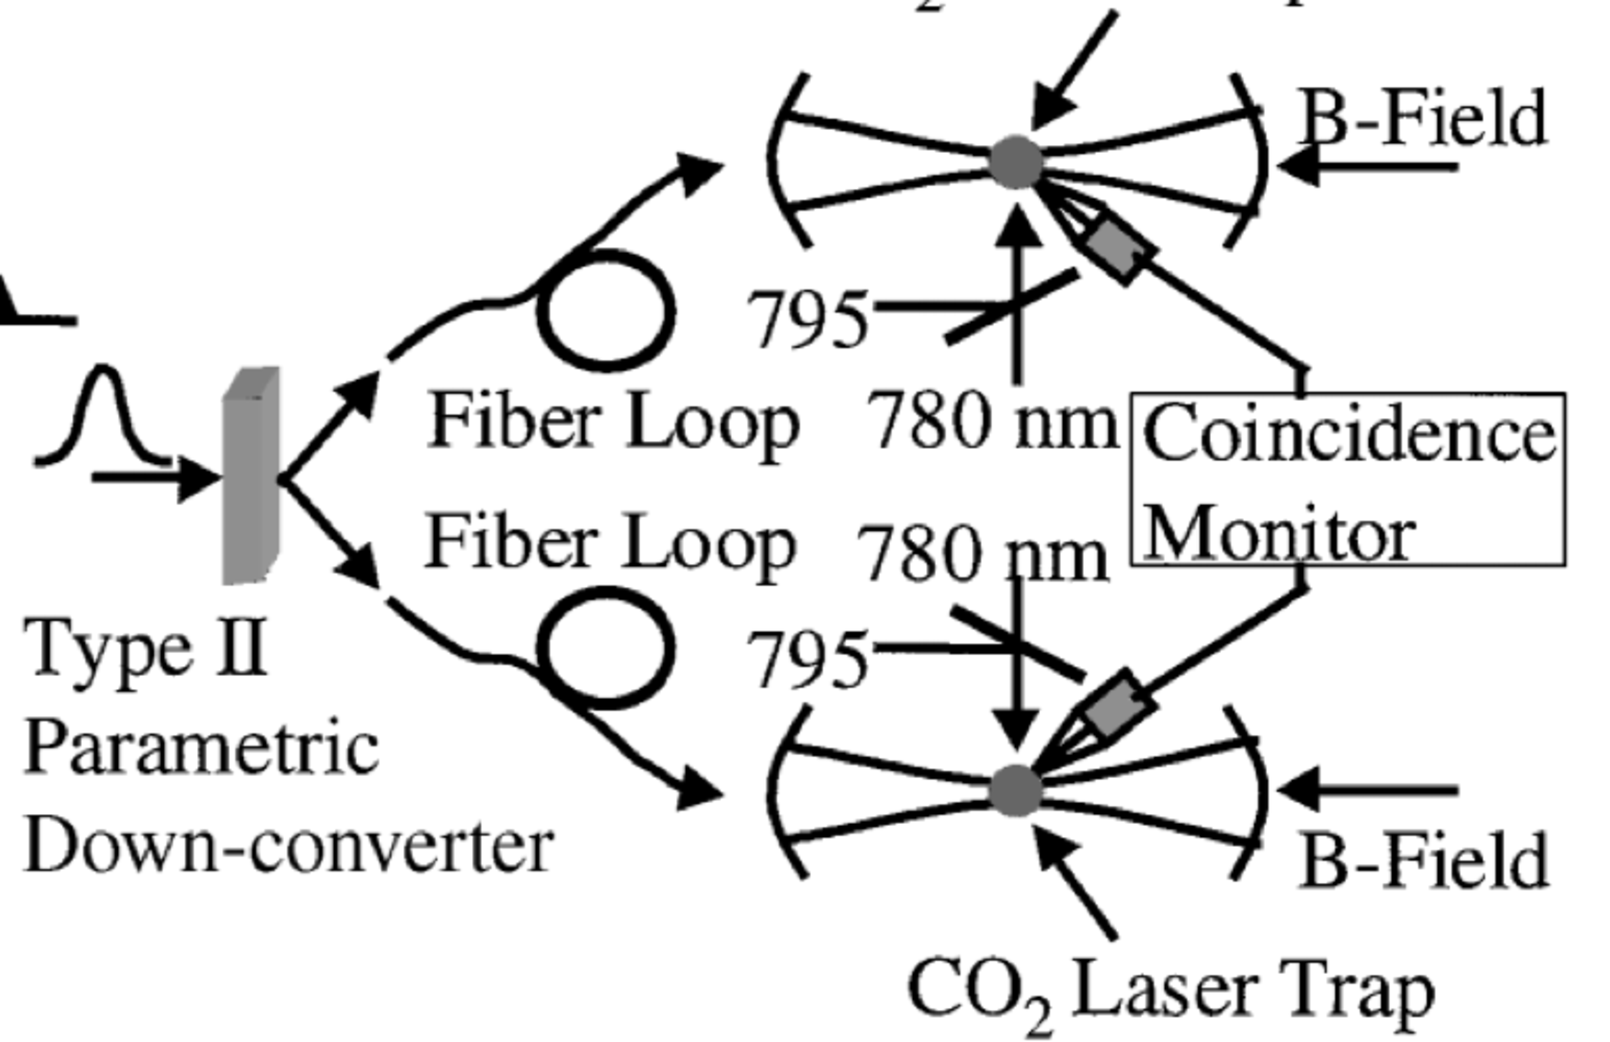
\includegraphics[width=0.39\textwidth]{figures/node}
  	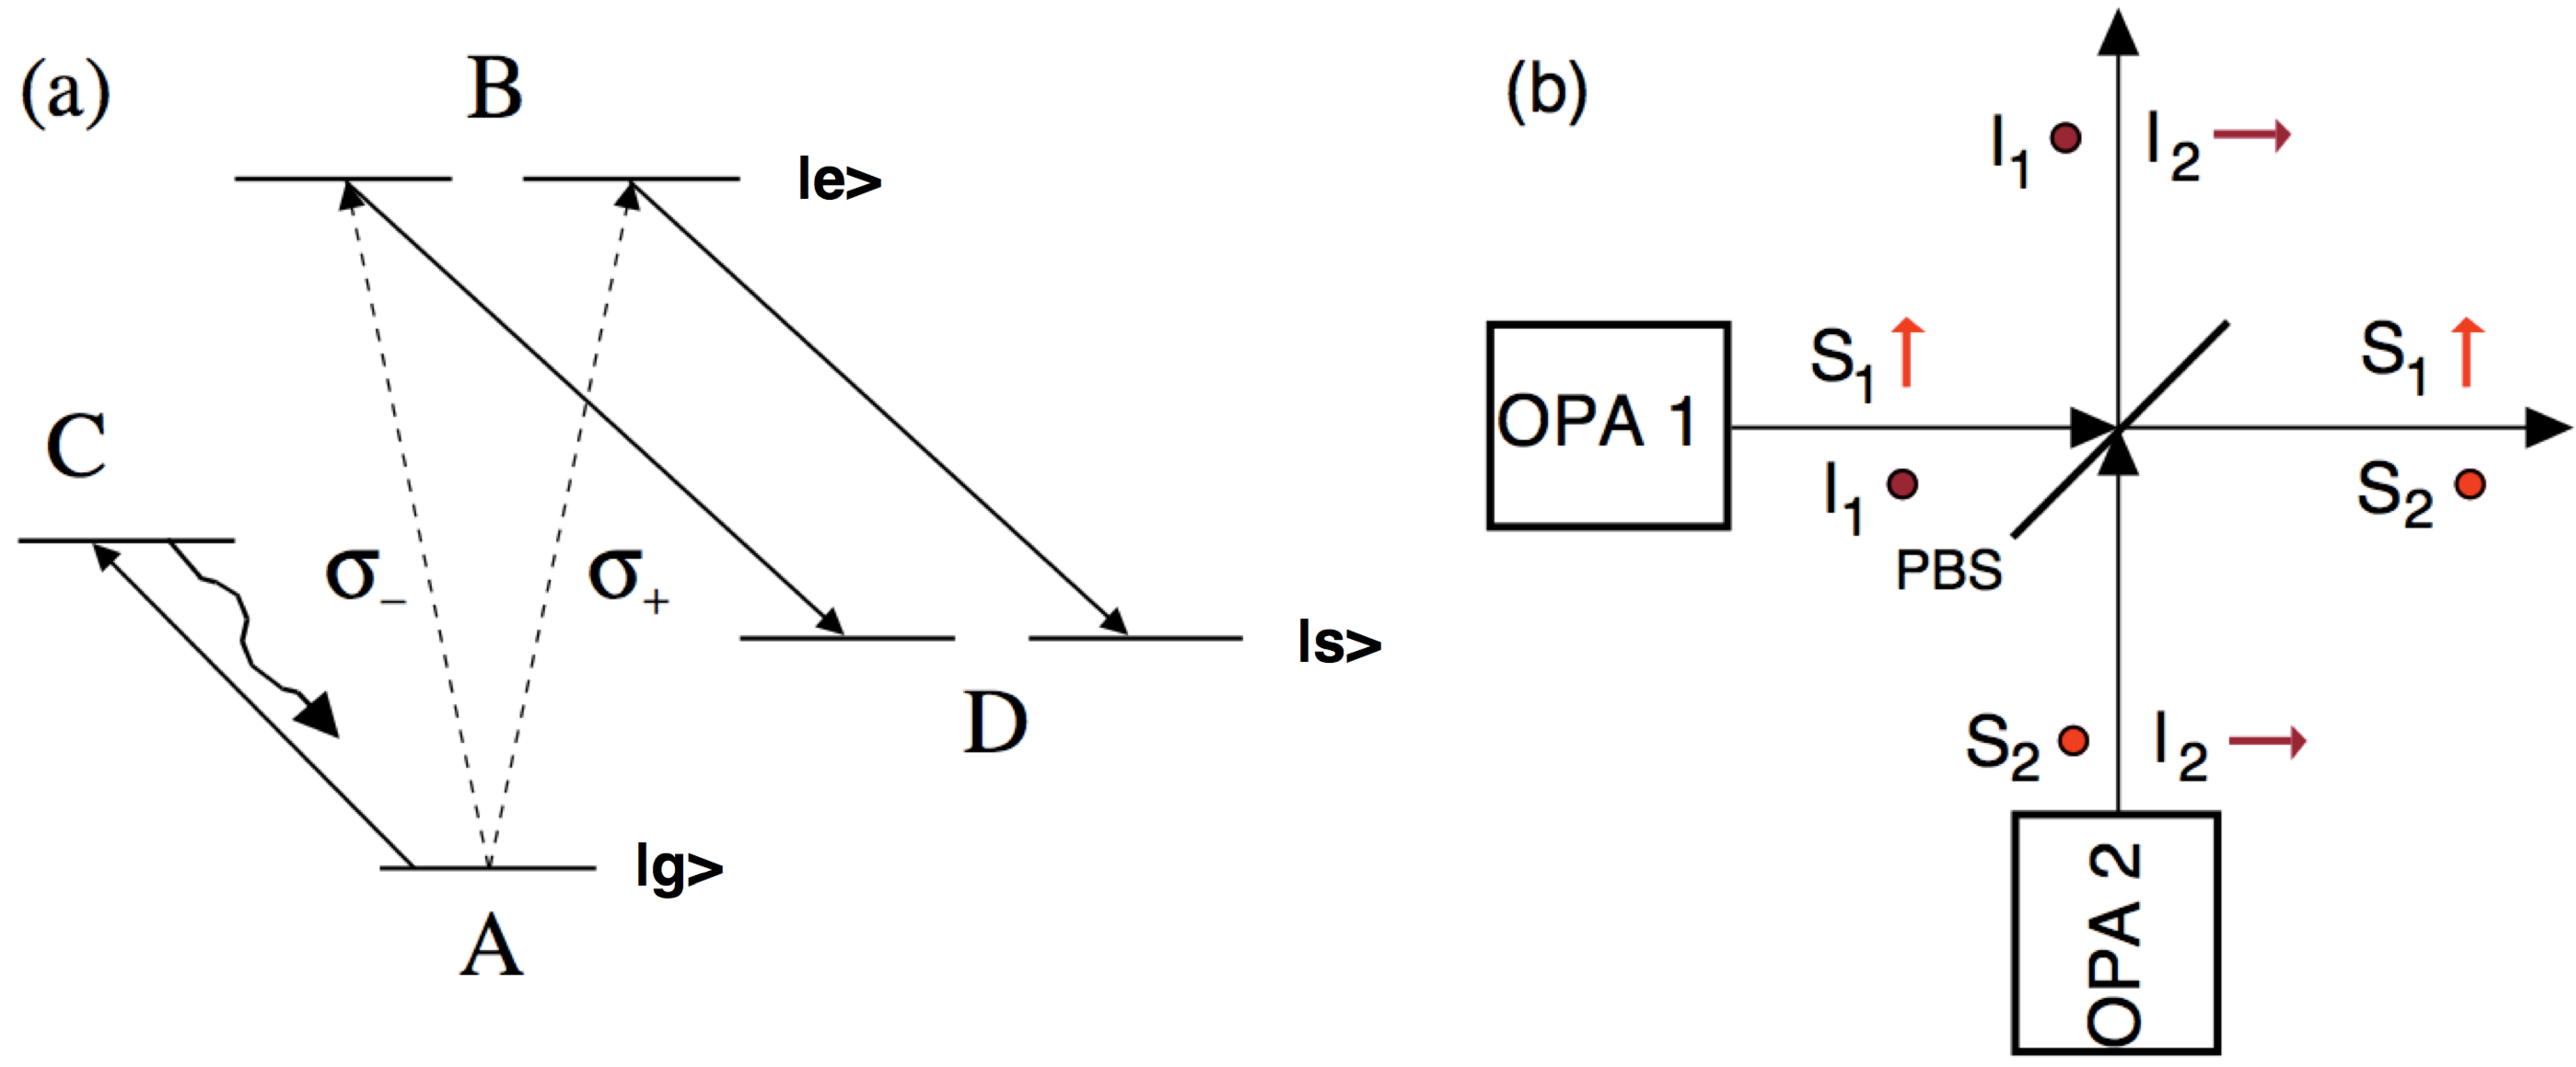
\includegraphics[width=0.50\textwidth]{figures/level_structure_opa1}
	\caption{Components of a quantum repeater node in the MIT-NU architecture. (a) Parametric downconversion creates pairs of polarization-entangled photons, sending the idler photon to atom-trap 1 and the signal photon to atom-trap 2. Each trap contains a single ultra-cold rubidium atom cooled to its hyperfine ground state. In the energy level diagram, the AB-transition absorbs 795 nm photons, and the BD-transition is coherently driven, thereby enabling storage at D. (b) Polarization-entangled photon pairs generated by a pair of type-II optical parametric amplifiers (OPAs) and a polarizing beam splitter (PBS). The polarizations $\hat{x}$ and $\hat{y}$ are denoted by arrows and bullets, respectively. Figures taken from~\cite{PhysRevLett.87.167903} and~\cite{1464-4266-2-1-101}.}
	\label{fig:diagram}
\end{figure}

\begin{figure}[t]
	\centering
	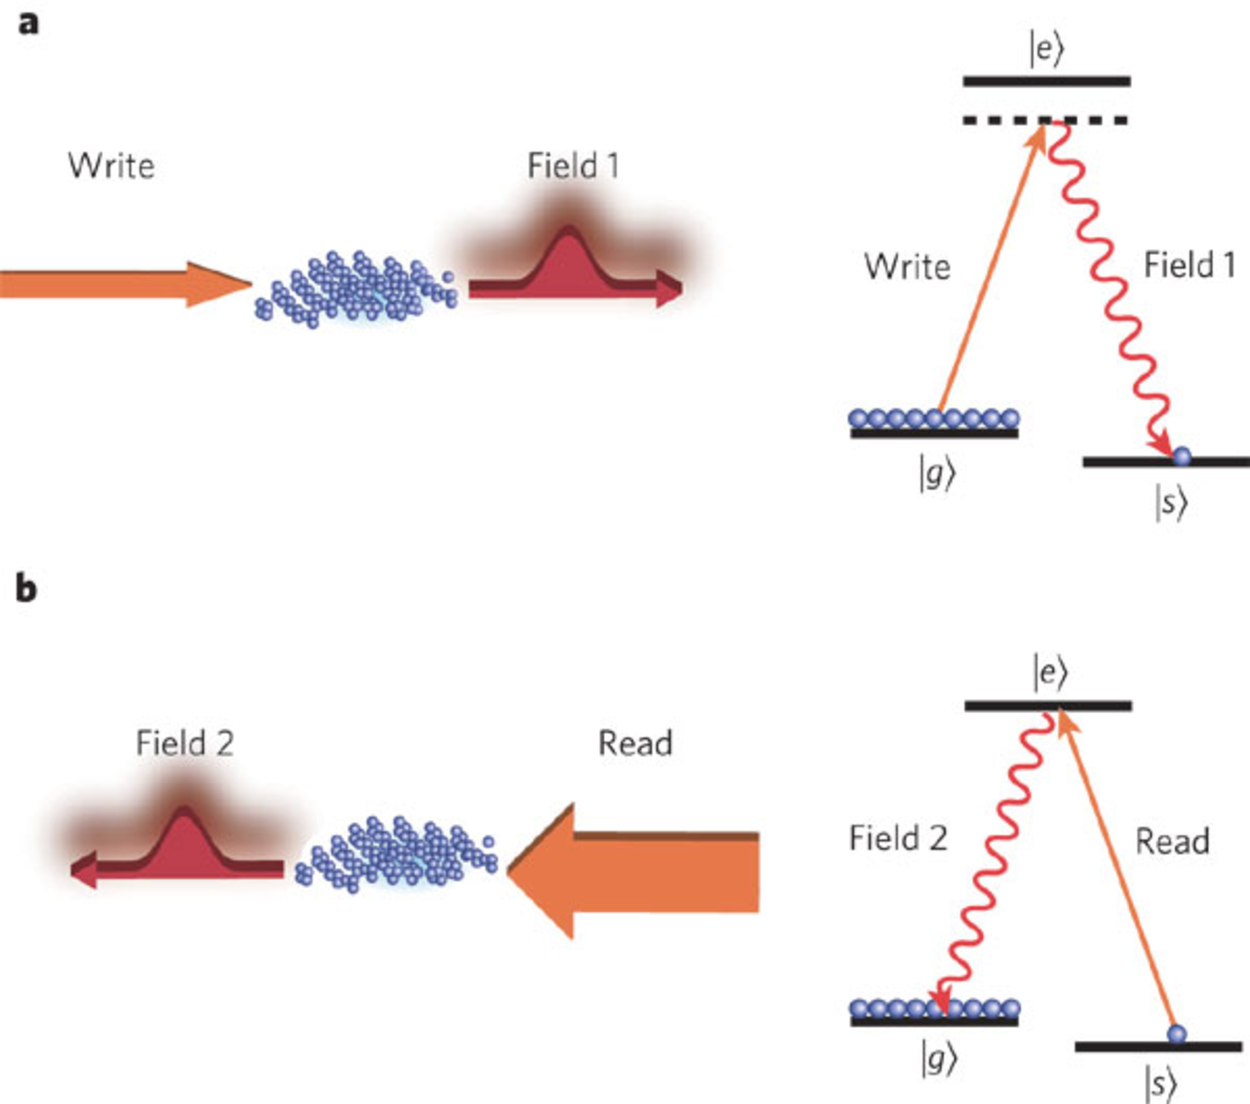
\includegraphics[width=0.40\textwidth]{figures/dlcz}
  	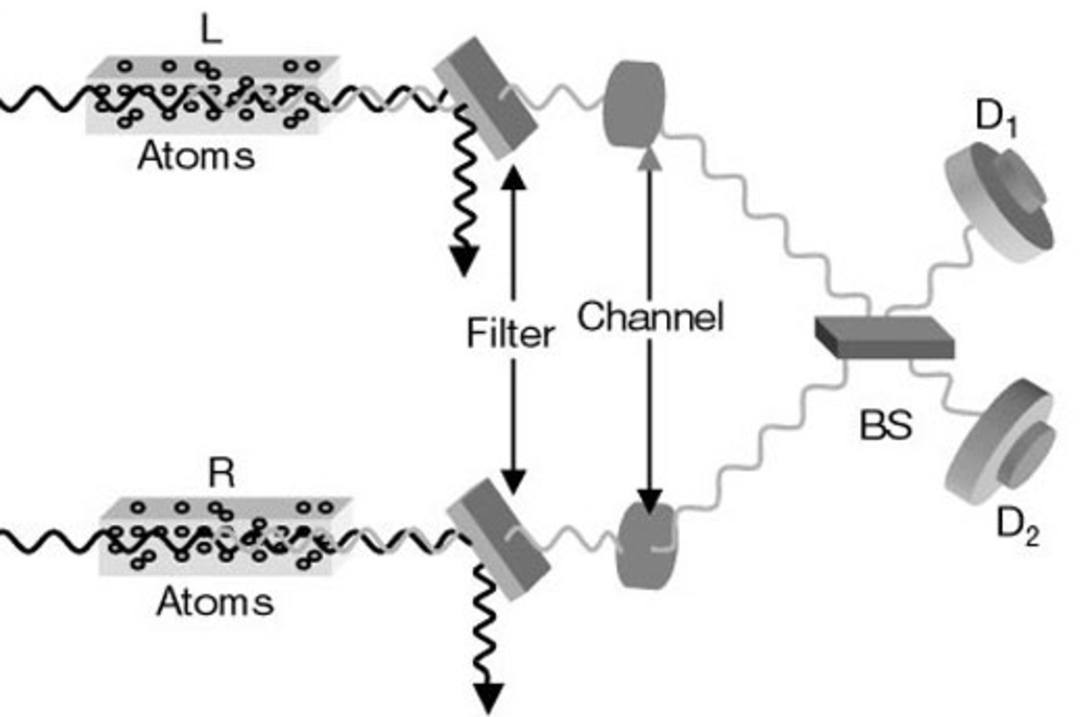
\includegraphics[width=0.50\textwidth]{figures/dlcz_entanglement}
	\caption{Entanglement with the DLCZ protocol. (Left) Weak and strong coherent pulses induce writing and and reading through spontaneous Raman transitions, respectively. (Right) Measurement-induced interference results in a single-excitation entangled state.  Figures taken from~\cite{nature07127} and~\cite{nature35106500}.}
	\label{fig:dlcz}
\end{figure}

An illustration of a model quantum communication system is shown in
Fig.~\ref{fig:diagram}, in the case of a single-trapped atom. Through type-II
parametric downconversion, a post-selected maximally-entangled state can be
produced of the form,
\eqn{
\ket{\psi_1} = \frac{1}{\sqrt{2}}\pna{\ket{\sigma_{+}}_1\ket{\sigma_{-}}_2 + e^{i\phi} \ket{\sigma_{-}}_1 \ket{\sigma_{+}}_2 } \label{eqn:singlet}
}
where $\sigma_{+}$ ($\sigma_{-}$) indicates right (left) circular polarization,
and $\phi$ is a phase offset. An arbitrary polarization of any photon entering
the cavity can be stored in the basis of right and left circular polarizations,
such that
\eqn{
\ket{\psi_2} = \alpha \ket{\sigma_{+}}+\beta \ket{\sigma_{-}}.
}
Through a Raman $\Lambda$-type interaction, a signal or idler photon
effectively transfers its entanglement to the degenerate B magnetic hyperfine
levels, and subsequently to the D levels through a coherently-driven
transition. However, the efficient coupling of a single photon to a single
trapped atom is a daunting technical task, requiring that the atom be held in
an ultrahigh-$Q$ cavity. By using an atomic ensemble, we eliminate the need for
such a high-quality cavity because a collective atomic state is easily produced
by a single photon. Such a state is one in which a single atom has been excited
from its ground state $\ket{g}$ at A to the metastable state $\ket{s}$ at D. 

To illustrate this behavior for an atomic ensemble, consider $N_a$ atoms
prepared in their ground states, a collective state denoted by
$\ket{0}_a=\ket{g}^{\otimes N_a}$. Coherently pumping the ensemble creates an
inelastic Raman scattering event that is collectively enhanced by constructive
interference within the ensemble~\cite{PhysRev.93.99}. The resulting
forward-scattered Stokes light arises from coherent spontaneous emission in the
ensemble, and the correlated ensemble excitation is a collective spin state,
\eqn{
\ket{1}_a = \hat{S}^{\dagger}\ket{0}_a=\frac{1}{\sqrt{N_a}}\sum_{i=1}^{N_a}\ket{g}_1\cdots\ket{s}_i\cdots\ket{g}_{N_a}.
\label{eq:dicke_state}
}
where $\hat{S}=(1/\sqrt{N_a})\sum_i\ket{g}_i\bra{s}$. Because the excitation is
composed of many atoms, the collective spin excitation is protected against the
loss of individual atoms in the ensemble, increasings its robustness for
storage. In the weak interaction limit, in which most of the atoms remain in
their ground state, the spin excitation $\hat{S}$ is effectively a ladder
operator, as $[\hat{S},\hat{S}^{\dagger}] =
\sum_i\pna{\ket{g}_i\bra{g}-\ket{s}_i\bra{s}}/N_a\approx 1$, and the outgoing
Stokes light and spin excitation are in a two-mode squeezed
state~\cite{nature35106500}. Generally, the term with the $n$th atom in
$\ket{s}$ acquires the phase $e^{i\pna{\mathbf{k}_w-\mathbf{k}_s}\cdot
  \mathbf{x}_n}$, where $\mathbf{k}_w$ is the wave vector of pump field,
$\mathbf{k}_s$ is that of the detected Stokes photon, and $\mathbf{x}_n$ is the
$n$th atom's position.  Collective excitations can be read out very efficiently
when converted into single anti-Stokes photons, which are emitted into a
well-defined mode because of collective interference. A resonant laser
excitation of the collective state in Eqn.~\ref{eq:dicke_state} results in
$N_A-1$ atoms in $\ket{g}$ and one delocalized excitation in $\ket{e}$. Through
decay to the $\ket{g}^{\otimes N_a}$, an anti-Stokes photon is emitted along
the $\ket{e}-\ket{g}$ transition. Denoting $\mathbf{k}_{as}$ and $\mathbf{k}_r$
as the wave vectors of the anti-Stokes photon and read laser, respectively,
satisfying the phase matching condition
$\mathbf{k}_{s}+\mathbf{k}_{as}=\mathbf{k}_{r}+\mathbf{k}_{w}$ results in a
very high probability amplitude for the anti-Stokes photon to be in the
$\mathbf{k}_{r}+\mathbf{k}_{w}-\mathbf{k}_{s}$ direction due to constructive
interference~\cite{PhysRevLett.103.043601}. 

Our analysis merges the approaches of trapped single atoms in cavity quantum
electrodynamics (QED) proposed by MIT and Northwestern University (MIT-NU) and
the ensemble-based repeater architecture proposed by Duan, Lukin, Cirac, and
Zoller (DLCZ)~\cite{PhysRevLett.87.167903,nature35106500}. The MIT-NU and DLCZ
protocols both utilize spontaneous Raman transitions to mediate atomic
storage. Whereas the MIT-NU protocol has the advantage of storing externally
generated entanglement and verifying its success through cycling-transition
fluorescence, it is prohibitively difficult to implement because of the strong
coupling requirements of cavity QED. 

In contrast, the DLCZ protocol creates a collective atomic excitation, as in
Eqn.~\ref{eq:dicke_state}, not by an external input photon, but by the ensemble
itself interacting with a classical (write) field. The entangled state is
generated probabilistically (but heralded) through postselection and
measurement quantum interference, as shown in Fig.~\ref{fig:dlcz}. In the ideal
case of low excitation probability, a photodetection event at either of the two
detectors projects the two ensembles into a maximally-entangled singlet state
of excitations. Although scalably resilient to issues that might plague such
protocols, such as propagation loss and photodetector dark counts, DLCZ
requires stable phase coherence and number-resolving photodetectors, neither of
which are easy to implement in practice. By enabling the storage of
externally-generated entanglement in a DLCZ-type protocol, we will address new
error models for entanglement fidelity in quantum memories.

\begin{figure}[t]
	\centering
	\resizebox{3.00in}{!}{\input cavity1.pdf_t}
	\resizebox{2.75in}{!}{\input raman1.pdf_t}
	%\input{cavity1.pdf_t}
	\caption{DLCZ with quantum field inputs. (Left) Input-output formalism for a single-sided, two-mode ring cavity. (Right) Interaction in a three-mode parametric amplifier}
	\label{fig:ours}
\end{figure}

We abstracted a model for the interaction of input quantum field into an
ensemble-based quantum memory. A basis for this model is inspired by recent
experimental work on heralded single-photon atomic memories and interfaces from
\cite{PhysRevLett.98.183601}~\cite{PhysRevLett.103.043601}, which utilized two
spatially-overlapping atomic ensembles to absorb arbitrarily polarized single
photons.  Heralding was observed (at rate of $10^{-6}$, using pulsed coherent
states ($\bar{N}\approx 500$) with an absorption probability
$\alpha=0.01$. Despite operating in an effective single-photon regime, multiple
photon inputs were still present, a problem we wish to analyze in the case of a
parametric downconverter input.  We consider an ensemble of $\Lambda$-type
atoms confined in a single-sided, low-finesse ring cavity, as shown in
Fig.~\ref{fig:ours}. The $\ket{g}-\ket{e}$ and $\ket{e}-\ket{s}$ transitions
are coupled to the cavity modes $\hat{a}$ and $\hat{b}$, respectively, each
with coupling coefficient $g_c$. Under the rotating wave approximation, the
interaction Hamiltonian for the collective interaction process is given by  
\eqn{
\hat{H} = \hbar\Gamma \pna{\hat{a}\hat{S}^{\dagger}\hat{b}^{\dagger} + \hat{b}\hat{S}\hat{a}^{\dagger}}\label{eq:trilinear}
}
where $\Gamma=g_c^2 N_a/\Delta$ ($\Delta$ is the detuning from the two-photon
resonance). In general, a Hamiltonian that cannot be analytically diagonalized
will not have analytical dynamics~\cite{theoretical_qoptics,group_qoptics}, and
will therefore not be useful in a Gaussian state analysis. A three-mode
interaction describes a heralding quantum memory where an input quantum field
(pump mode $\hat{a}$) creates a stationary ensemble excitation (idler mode
$\hat{b}$) and a heralding Stokes photon (signal mode
$\hat{S}$). Parameterizing the strength of this interaction by $\Gamma$, the
trilinear Hamiltonian describing this process is then
\eqn{
\hat{H}=\hat{H}_0+\hat{H}_{\textrm{int}}\label{eq:tri_h_total}
}
where
\eqn{
\hat{H}_0=\omega_a \hat{a}^{\dagger}\hat{a}+\omega_b \hat{b}^{\dagger}\hat{b}+\omega_S \hat{S}^{\dagger}\hat{S}
}
\eqn{
\hat{H}_{\textrm{int}}=\Gamma
\hat{a}\hat{b}^{\dagger}\hat{S}^{\dagger}+\Gamma^*
\hat{S}\hat{b}\hat{a}^{\dagger} \label{eqn:final_tri_ham}
}
with 
\eqn{
\pnb{\hat{H}_0, \hat{H}_{\textrm{int}}}=0. 
}
assuming that each mode begins from rest, we can also say that 
\eqn{
\hat{N}_{abc}= 2\hat{a}^{\dagger}\hat{a}+\hat{b}^{\dagger}\hat{b} +\hat{S}^{\dagger}\hat{S} \qquad \hat{N}_{bc}=\hat{b}^{\dagger}\hat{b}-\hat{S}^{\dagger}\hat{S}
}
are conserved quantities. In Section~\ref{chap:herald}, we assume an
\emph{anzatz} solution such that $N$ entangled photons are absorbed by an
ensemble memory and are converted, without loss, to $N$ spin excitations and
$N$ heralding photons.  Note that that operations preserving the Gaussian
properties of a quantum state's Wigner function (e.g., for
polarization-entangled light) must be quadratic in its boson operator
terms~\cite{RevModPhys.77.513}. Any quadratic interaction Hamiltonian is thus a
Gaussian operation, and the solutions for its input-output behavior is a
Bogoliubov transformation of the input modes. However, it is not even possible
to determine the analytical dynamics for Eqn.~\ref{eqn:final_tri_ham}, because
it is not a quadratic Hamiltonian. In the following section, we will describe
some subtleties and prospects for achieving strong interactions between
quantized excitations, in the trilinear case.

We can compensate for finite detunings and heralding probabilities in these
ensembles by increasing the ensemble's optical depth, which is limited in
free-space interactions by ensemble size and coupling strength. Several
approaches use multi-pass optical cavities to increase the likelihood of a
successful Raman scattering event between a cavity field and the enclosed
ensemble~\cite{PhysRevLett.92.123601, PhysRevLett.95.133601,
  PhysRevLett.98.190503,Thompson07072006,PhysRevLett.98.183601}. The
cavity-ensemble heralding efficiency is captured by the cooperativity parameter
$C=g_c^2 N_A/\kappa_c \gamma$ , where $g_c$ is the single-atom coupling
constant to the cavity mode, $\kappa_c$ is the cavity decay rate, and $\gamma$
is the excited state spontaneous decay rate. It can be shown that the
cooperativity is approximately $C\sim fd$, where $d$ is the optical depth of
the ensemble and the finesse ${f}$ is approximately the number of passes the
optical field makes in the cavity. Optical cavities are used in the magnon-type
memory, in which a single collective excitation is shared between between two
spatially-overlapping atomic ensembles ~\cite{PhysRevLett.103.043601}. Photons
of arbitrary polarization states are stored between two ensembles that absorb
only left- ($\sigma^{+}$) and right-circularly ($\sigma^{-}$) polarized light,
respectively, and emit only linearly ($\pi$) polarized light into the cavity
resonator, thereby eliminating any which-path information. The memory itself is
an ensemble of approximately 8000 cesium atoms loaded from a far-detuned
magneto optical trap (MOT) into a one-dimensional optical lattice overlapping a
medium-finesse ($f=140$) optical cavity. A spatially homogenous, DC magnetic
field allows time-dependent control of polarization storage through Larmor
precession of the ensembles magnetic moment. In theory, single-photon
conversion efficiencies for this type of magnon memory are quite high.

As an aside, it is worth noting a competing approach to photon storage that may
serve as a useful comparison in the future, namely, the usage of stimulated
Raman transitions and electromagnetically induced transparency (EIT) to
increase the coupling of an input quantum field with an atomic
ensemble~\cite{PhysRevA.65.022314,RevModPhys.75.457,PhysRevLett.98.123601,PhysRevA.76.033804}. In
this approach, an external coherent control field couples the $\ket{e}-\ket{s}$
transition in a $\Lambda$-type atom, adiabatically reducing the group velocity
of a single photon wavepacket and trapping it within the ensemble. Such an
approach is deterministic, with high throughput, but admits neither easy
verification (as in MIT-NU) nor heralding (as in DLCZ). Like the DLCZ protocol
above, its compatibility with externally-generated entanglement is an open
question.


\subsection{Polarization Quantum Entanglement and Communication\label{sec:intro:entanglement}}

Because we will be concerned with the behavior of atomic ensembles that are
illuminated by the entangled signal and idler produced by optical parametric
amplification (OPA), it is important to have an appropriate model for such
light beams. As our goal is to quantify the effects of multiple-pair emissions
from such a source on the resulting stored entanglement, we cannot immediately
default to a postulated biphoton picture. Instead, we shall use the full
Gaussian-state description, in which the the input field in this interaction is
one of a pair of polarization-entangled light beams generated by the
interference of a pair of anti-phased optical parametric amplifiers as shown in
Fig.~\ref{fig:diagram}. We assume that the signal and idler cavities are
matched with identical linewidths $\Gamma$, and pumping fractions, $G^2$, of
oscillation threshold, with no depletion of or excess noise on the
pump~\cite{1367-2630-4-1-347, 1464-4266-2-1-101}. Following interference, the
output fields are in an entangled, zero-mean Gaussian pure state with the
normally-ordered and phase-sensitive correlation functions
\begin{align}
&\langle \hat{A}^{\dagger}_{k_j}\pna{t+\tau} \hat{A}_{k_j}\pna{t}\rangle = \frac{G \Gamma}{2} 
\pnb{\frac{e^{-\pna{1-G}\Gamma \abs{\tau}}}{1-G}-\frac{e^{-\pna{1+G}\Gamma \abs{\tau}}}{1+G}}\nonumber \\
&\langle \hat{A}_{S_j}\pna{t+\tau} \hat{A}_{I_j}\pna{t}\rangle \nonumber \\ 
& \qquad =\frac{\pna{-1}^{j-1}G \Gamma}{2} 
\pnb{\frac{e^{-\pna{1-G}\Gamma \abs{\tau}}}{1-G}+\frac{e^{-\pna{1+G}\Gamma \abs{\tau}}}{1+G}},	
\end{align}
where $\{\hat{A}_{k_j}\pna{t}e^{-j\omega_k
  t}:~k=S\pna{\textrm{signal}},I\pna{\textrm{idler}},j=1,2\}$ are the positive-frequency, photon-units OPA-output fields. The low-flux output state
of this process at a detuning $\Delta \omega$ is given by expanding out the
number ket representations of the OPAs to first order,
\begin{align}
\ket{\psi}_{\textrm{SI}} & = \sum_n
\sqrt{\frac{\bar{N}}{\pna{\bar{N}+1}^{n+1}}} \ket{n}_{S_x}\ket{n}_{I_y}
\nonumber \\ & \qquad \otimes \sum_n \pna{-1}^n \sqrt{\frac{\bar{N}}{\pna{\bar{N}+1}^{n+1}}} \ket{n}_{S_y}\ket{n}_{I_x} \nonumber \\
%& \approx\frac{1}{\bar{N}+1} \ket{0}_{S_x}\ket{0}_{I_y}\ket{0}_{S_y}\ket{0}_{I_x}+ \sqrt{\frac{\bar{N}}{\pna{\bar{N}+1}^{3}}}\pna{\ket{1}_{S_x}\ket{1}_{I_y}\ket{0}_{S_y}\ket{0}_{I_x}-\ket{0}_{S_x}\ket{0}_{I_y}\ket{1}_{S_y}\ket{1}_{I_x}}\nonumber \\
& \approx \ket{\textrm{vac}}+\sqrt{\frac{\bar{N}}{\pna{\bar{N}+1}^{3}}}\pna{\ket{H}_S\ket{V}_I-\ket{V}_S\ket{H}_I},\label{eq:final_singlet}
\end{align}
where $\bar{N}=4G^2/\pnb{\pna{1-G^2-\Delta
    \omega^2/\Gamma^2}^2+4\Delta\omega^2/\Gamma^2}$ is the average photon
number per mode; and $\ket{H}_S=\ket{1}_{S_x}\ket{0}_{S_y}$,
$\ket{V}_S=\ket{0}_{S_x}\ket{1}_{S_y}$, $\ket{H}_I=\ket{1}_{I_x}\ket{0}_{I_y}$,
and $\ket{V}_I=\ket{0}_{I_x}\ket{1}_{I_y}$. Following measurement
postselection, this state is a maximally entangled singlet state of the form in
Eqn.~\ref{eqn:singlet}~\cite{1367-2630-4-1-347}, and expansions to higher
orders account for multiple-pair effects. A useful property of the full state
$\ket{\psi}_{\textrm{SI}}$ is that its anti-normally ordered characteristic
function is a zero-mean, jointly Gaussian distribution that remains Gaussian
under linear transformations. Its joint density operator is
$\hat{\rho}_{SI}=\hat{\rho}_{S_x I_y}\otimes\hat{\rho}_{S_y I_x}$, whose
anti-normally ordered characteristic functions are given by
\begin{align} 
\chi_A^{\rho_{S_x I_y}}\pna{\zeta_S,\zeta_I} & = \langle e^{-\zeta_S^* \hat{a}_{S_x}-\zeta_I^* \hat{a}_{I_y}} e^{\zeta_S \hat{a}_{S_x}^{\dagger}+\zeta_S \hat{a}_{I_y}^{\dagger}} \rangle \nonumber \\
& = e^{-\pna{1+\bar{N}}\pna{|\zeta_S|^2+|\zeta_I|^2}+2\bar{N}\textrm{Re}\pna{\zeta_S \zeta_I}}
\end{align}
and 	
\begin{align}
\chi_A^{\rho_{S_y I_x}}\pna{\zeta_S,\zeta_I} & = \langle e^{-\zeta_S^* \hat{a}_{S_y}-\zeta_I^* \hat{a}_{I_x}} e^{\zeta_S \hat{a}_{S_y}^{\dagger}+\zeta_I \hat{a}_{I_x}^{\dagger}} \rangle \nonumber \\
& = e^{-\pna{1+\bar{N}}\pna{|\zeta_S|^2+|\zeta_I|^2}-2\bar{N}\textrm{Re}\pna{\zeta_S \zeta_I}},
\end{align}
which contain all multiple-pair orders of $\ket{\psi}_{\textrm{SI}}$. Following
a linear transformation, the output state $\hat{\rho}_{\textrm{out}}$ can be
determined by taking the inverse Fourier transform of the output characteristic
function, with that characteristic function being easily calculated from the
input characteristic function and the field transformation. In a memory or
teleportation architecture, we want the output---represented by a pure or mixed
state $\hat{\rho}_{\textrm{out}}$--- to have the highest possible fidelity with
respect to its input state $\hat{\rho}_{\textrm{in}}$. The trace separation
quantifies this fidelity as
$F\pna{\hat{\rho}}=\textrm{Tr}\pnb{\sqrt{\hat{\rho}_{\textrm{out}}}\hat{\rho}_{\textrm{in}}
  \sqrt{\hat{\rho}_{\textrm{out}}}}$, which reduces to a projection overlap
${\bra{\psi_{\textrm{in}}} \hat{\rho}_{\textrm{out}} \ket{\psi_{\textrm{in}}}}$
when the input is the pure state
$\hat{\rho}_{\textrm{in}}=\ket{\psi_{\textrm{in}}} \bra{\psi_{\textrm{in}}}$.

\begin{figure}[t]
\centering
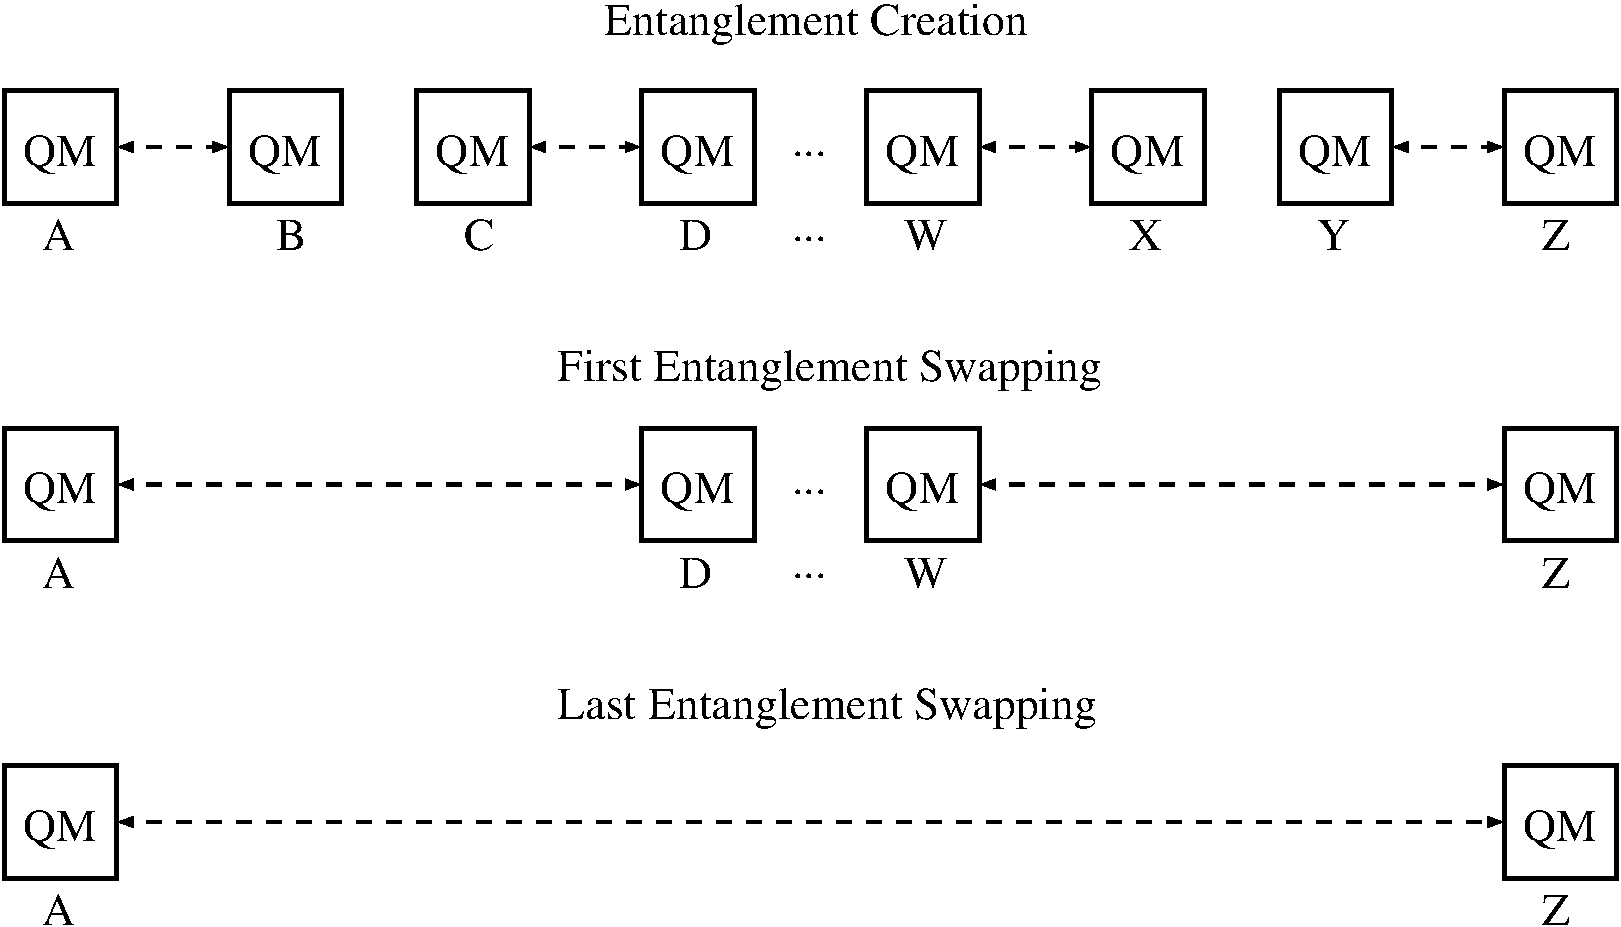
\includegraphics[width=0.50\textwidth]{figures/connection.pdf}
\caption{\label{fig:chap1:connection} Principle of a quantum repeater architecture. Entanglement is independently created at short distances between nodes $\textrm{AB}\ldots\textrm{YZ}$. Entanglement is swapped between neighboring links such that locations A and D, for example, share entanglement over an intermediate distance. Swapping occurs over successively larger distances until links at the desired separation, A and Z, are entangled. Figure based on~\cite{2009arXiv0906.2699S}.}
\end{figure}

The most immediate problem affecting the distribution of polarization-entangled
photons is photon propagation loss. Although a 1 km length of low-loss, optical
telecom fiber ($\lambda = 1.55~\mu m$)---a relatively short distance---has a
transmission nearing 95\%, photon transmission decays exponentially with
increasing distances, ruling out direct transmission of entangled photons over
hundreds of kilometers. In classical communication, this type of signal
attenuation is easily compensated with fiber-based amplifiers. However, for
quantum communication, the no-cloning theorem prevents noiseless amplification
of the non-orthogonal quantum states required for
teleportation~\cite{citeulike:507853}.

Fig.~\ref{fig:chap1:connection} shows a `quantum repeater' approach that
overcomes the amplifier restriction by incrementally extending entanglement
across a larger network~\cite{2009arXiv0906.2699S}. Lettered boxes represent
memories, and pairs of memories form nodes on the network. For two nodes, A---B
and C---D, that are each separately entangled, a joint Bell measurement between
memories B and C will entangle systems A and D. This process, known as
\emph{entanglement swapping}, establishes entanglement between two networks
links that may have never interacted. One can then establish entanglement
between memories A and Z that are separated by a distance $L$ by independently
creating entanglement at $N$ equally-spaced adjacent nodes out of $2N$
memories. $N-1$ entanglement swapping operations in this network ultimately
entangle memories A and Z. For the repeater protocol to work in an asynchronous
fashion, these links must be heralding quantum memories. Together,
entanglement repeaters and teleportation form basis for high-fidelity
communications of quantum states over long distances.

\begin{comment}

  Once entanglement distribution is successful, we can carry out long-distance
  quantum communication using teleportation, a protocol described in
  Fig.~\ref{fig:chap1:teleportation}. In qubit teleportation, Charlie (C) sends
  a message (M) to Bob (B) using Alice (A) as an intermediary. Charlie's
  message is in the form of an arbitrary, unknown qubit spanned by the
  orthonormal basis $\{\ket{0},\ket{1}\}$ represented by $\ket{\psi}_C=\alpha
  \ket{0}_C+\beta\ket{1}_C$, where $\abs{\alpha}^2+\abs{\beta}^2=1$. Together,
  entanglement repeaters and teleportation form basis for high-fidelity
  communications of quantum states over long distances.

\end{comment}




% Theory Results
\section{Heralded Polarization Entanglement Distribution with Atomic
  Ensembles\label{chap:herald}}

This section combines the operating principles of ensemble-based quantum
memories with architectures for polarization entanglement distribution,
entanglement connection, and quantum teleportation. We will first discuss our
architecture for entanglement distribution and provide a very basic abstraction
for quantum memories. The remainder characterizes figures of merit---fidelity,
heralding probability, and protocol success probability---under various
transmission loss and photodetection conditions.

\subsection{Architecture Overview and Figures of Merit\label{sec:herald:overview}}

\begin{figure*}[t]
	\centering
	\resizebox{6.50in}{!}{\input spdc_dlcz_fin.pdf_t}
	\caption{Modified DLCZ architecture for distributing polarization entanglement, using a spontaneous parametric downconversion (SPDC) source and  interferometer measurement for entanglement verification.}
	\label{fig:channel_model}
\end{figure*}

\begin{figure*}[htb]
	\centering
	\resizebox{6.50in}{!}{\input spdc_dlcz_loss.pdf_t}
	\caption{Hong-Ou-Mandel (HOM) interferometer measurement with loss (labeled).}
	\label{fig:channel_loss_model}
\end{figure*}

We will first discuss our overall architecture and loss model, followed by
particular details of a dual-OPA polarization entanglement source and quantum
memories. Our architecture for polarization entanglement distribution, shown in
Fig.~\ref{fig:channel_model}, is a modification of the standard DLCZ
architecture shown in Fig.~\ref{fig:dlcz}. In the original DLCZ protocol, both
ensembles are coherently pumped and the probability that both ensembles will
emit single photons is low compared to that for emission from a single
ensemble. Interference at the 50-50 beam splitter in Fig.~\ref{fig:dlcz} erases
any which-path information for the emission event, so a single detection at
either photon counter $D_1$ or $D_2$ is used to herald entanglement of the two
ensembles. The ideal situation in Fig.~\ref{fig:channel_model} is when a
polarization singlet is emitted from the source and the overall system is
lossless. The polarizing beam splitters (PBS) then load the signal and idler
photons from the singlet into a coherent superposition of excitations of
ensembles 1 and 2 and ensembles 3 and 4, respectively. This loading is heralded
by the single-photon detections from pair $\pna{D_1, D_2}$ and $\pna{D_3,
  D_4}$.

Fig.~\ref{fig:channel_loss_model} encompasses the error modes for the
Fig.~\ref{fig:channel_model} distribution architecture. The Type-II SPDC source
may produce multiple signal-idler pairs, which will be modeled with the full
joint Gaussian state description of its output. Propagation losses between the
PBS and the atomic ensembles (labelled `pre'), and between the atomic ensembles
and the 50-50 beam splitter (labelled `post') are modeled by fictitious beam
splitters whose vacuum-state input ports inject Gaussian quantum noise. Finite
quantum efficiency photodetectors (labelled `pho') are similarly modeled, and
we have ignored dark counts, which are known to be reasonably low at heralding
wavelengths for silicon Geiger-mode avalanche photodiodes
(APDs)~\cite{Thomas2010}. Our number state model for these fictitious beam
splitters, described in Section~\ref{sec:herald:number}, includes the effects
of phase differences between input ports, which we can use to characterize the
effects of phase mismatch between pairs of ensembles. We will assume that any
accumulated phase offsets leading to the ensembles can be incorporated into the
pre-transmission efficiency.

The preceding imperfections expose two fundamentally different failure modes
for this protocol that affect fidelity and probability of success,
respectively. First, is it possible for heralding detections at the APDs to
declare the protocol's success even when the ensembles themselves are not in a
polarization singlet state. For example, a multiple-pair event from the
entanglement source could lead to multiple heralding photons emitted by a
quantum memory. Post-memory attenuation and finite-quantum efficiency
photodetection could eliminate all but one of those heralding photons, and the
usage of Geiger-mode APDs might completely preclude our ability to distinguish
between multiple-photon and single-photon events. A relative phase offset
between two ensembles, either because of pump photon phase mismatch or
pre-transmission phase accumulation, would similarly affect the final fidelity
of the loaded quantum state. Lastly, because post-memory imperfections reduce
potential heralding detections, it possible to declare the protocol a
failure---and reduce the probability of success---even when the ensembles are
successfully loaded.

We characterize this architecture's performance of heralding entanglement
distribution by determining its fidelity figure-of-merit and measurement
statistics under different photodetection schemes: photon-number resolving
detection (PNRD), which can distinguish between single-photon and multi-photon
photodetection events; and non-resolving single-photon detection (NRPD), which
is unable to exclude multi-photon error events. For these two schemes, the
projective measurement operators $\hat{M}_j~\pna{j=1,2,3,4}$ represent four
successful heralding outcomes at the photodetectors $D_i~\pna{i=1,2,3,4}$. The
input to each 50-50 beam splitter in Fig.~\ref{fig:channel_model} is a
superposition state of linearly co-polarized heralding photons from the atomic
memories, so we expect that successful entanglement distribution to yield
single clicks at the signal and idler photodetector pairs. This DLCZ-like
protocol for heralded polarization entanglement distribution therefore requires
the occurrence of a single detection on either photodetectors $D_1$ or $D_2$,
as well as a \emph{corresponding event} on either $D_4$ or $D_3$. In the
following, successful heralding is given by the projective measurements

\begin{widetext}
\begin{align}
    \hat{M}_j^{\textrm{PNRD}} = \left\{
	\begin{array}{lr}
\pna{\ket{1}_{11}\bra{1}}\otimes\pna{\ket{0}_{22}\bra{0}}\otimes\pna{\ket{1}_{33}\bra{1}}\otimes\pna{\ket{0}_{44}\bra{0}} & j=1\\
\pna{\ket{0}_{11}\bra{0}}\otimes\pna{\ket{1}_{22}\bra{1}}\otimes\pna{\ket{1}_{33}\bra{1}}\otimes\pna{\ket{0}_{44}\bra{0}} & j=2\\
\pna{\ket{0}_{11}\bra{0}}\otimes\pna{\ket{1}_{22}\bra{1}}\otimes\pna{\ket{0}_{33}\bra{0}}\otimes\pna{\ket{1}_{44}\bra{1}} & j=3\\
\pna{\ket{1}_{11}\bra{1}}\otimes\pna{\ket{0}_{22}\bra{0}}\otimes\pna{\ket{0}_{33}\bra{0}}\otimes\pna{\ket{1}_{44}\bra{1}} & j=4
	\end{array}
	\right.,
\end{align}


\begin{align}
    \hat{M}_j^{\textrm{NRPD}} = \left\{
	\begin{array}{lr}
\pna{\hat{I}_1-\ket{0}_{11}\bra{0}}\otimes\pna{\ket{0}_{22}\bra{0}}\otimes\pna{\hat{I}_3-\ket{0}_{33}\bra{0}}\otimes\pna{\ket{0}_{44}\bra{0}} & j=1\\
\pna{\ket{0}_{11}\bra{0}}\otimes\pna{\hat{I}_2-\ket{0}_{22}\bra{0}}\otimes\pna{\hat{I}_3-\ket{0}_{33}\bra{0}}\otimes\pna{\ket{0}_{44}\bra{0}} & j=2\\
\pna{\ket{0}_{11}\bra{0}}\otimes\pna{\hat{I}_2-\ket{0}_{22}\bra{0}}\otimes\pna{\ket{0}_{33}\bra{0}}\otimes\pna{\hat{I}_4-\ket{0}_{44}\bra{0}} & j=3\\
\pna{\hat{I}_1-\ket{0}_{11}\bra{0}}\otimes\pna{\ket{0}_{22}\bra{0}}\otimes\pna{\ket{0}_{33}\bra{0}}\otimes\pna{\hat{I}_4-\ket{0}_{44}\bra{0}} & j=4
	\end{array}
	\right.,
	\label{eq:chap3:meas_povm}
\end{align}
\end{widetext}
where $\ket{n}_i$ ($n=0,1$) are the vacuum and single-photon states, and
$\hat{I}_i$ is the identity operator for the $\hat{a}_i$ mode measured at
photodetector $D_i$ ($i=1,2,3,4$).

The heralding probability $P_{\textrm{herald}}$ is the probability a
heralding---a $\pna{D_1, D_2}$ single slick and a $\pna{D_3, D_4}$ single
click. The success probability $P_{\textrm{success}}$ is the probability that
heralding has occurred and the four ensembles have loaded a polarization Bell
state. The fidelity $F_j$ is the projection of the post-heralding ensemble
state onto the appropriate Bell state for $\hat{M}_j$ heralding, i.e.,
\begin{align}
\ket{\psi_j} & 
=
\frac{1}{\sqrt{2}}\pna{\ket{1}_S^1\ket{0}_S^2\ket{0}_S^3\ket{1}_S^4+\pna{-1}^j
  \ket{0}_S^1\ket{1}_S^2\ket{1}_S^3\ket{0}_S^4} \nonumber \\ & \qquad \qquad
\qquad \qquad \pna{j=1,2,3,4}.\label{eqn:remaining_singlet}
\end{align}
Following a photodetection measurement, the joint density operator of the four
atomic ensembles is determined by applying $\hat{M}_j$ and tracing over the
optical modes:
	\eqn{
	\hat{\rho}_{\textrm{post}}^j=\frac{1}{P_j^{\textrm{herald}}}\textrm{tr}_{1,2,3,4}\pna{\hat{\rho}_{\textrm{out}}\hat{M}_j}
	}
	where $\hat{\rho}_{\textrm{out}}$ is the joint density operator of the heralding light fields and the ensembles 
	\eqn{
	P_j^{\textrm{herald}}=\textrm{tr}\pna{\hat{\rho}_{\textrm{out}}\hat{M}_j} \label{eqn:herald_prob}.
}
If $\ket{\psi_j}$ is the entangled state of the four ensembles as heralded by
$\hat{M}_j$, and the entanglement storage fidelity is $F_j$, we find that the
success probability is
\eqn{
P_{\textrm{success}} = \sum_{j=1}^4 P_j^{\textrm{herald}} F_j =\sum_{j=1}^{4} \textrm{tr}\pna{\hat{\rho}_{\textrm{out}}\hat{M}_j} \bra{\psi_j} \hat{\rho}_{\textrm{post}}^j \ket{\psi_j}.\label{eq:success_prob_def}  
}
We will determine these measurement statistics using a full number-state
analysis. Because the successful heralding outcomes defined by $\hat{M}_j$ are
symmetric, all the fidelities $F_j$ are equal to each other. We will,
therefore, calculate only $F_1$ without any loss of generality.  In what
immediately follows, we will formalize our approach for calculating the joint
density operator of the light-ensemble system following entanglement
distribution.

\subsection{Photon Number Probability Distributions}

\begin{figure}[tb]
	\centering
	\resizebox{3.00in}{!}{\input beamsplitter.pdf_t}
	\caption{Beam splitter action on an input density operator $\hat{\rho}_{\textrm{in}}$ with two input ports and two output ports. Labeled at each port are the input and output bases used in Eqns.~\ref{eqn:chap3_rho_input} and~\ref{eqn:chap3_rho_output}. The boson annihilation operations at the input and output are $\hat{a}_i$ and $\hat{b}_i$, respectively, and the accompanying index $i$ represents signal ($i=1$) and auxiliary modes ($i=2$).}
	\label{fig:beamsplitter_model}
\end{figure}

Our first task is to concisely represent the effects of propagation loss on
light beams of arbitrary statistical composition, as shown by the unitary beam
splitter transformation in Fig.~\ref{fig:beamsplitter_model}.  The matrix
representation of linear-loss beam splitters in
Fig.~\ref{fig:channel_loss_model} corresponds to the $\textrm{SU}\pna{2}$ Lie
group representation from angular momentum
quantization~\cite{PhysRevA.40.1371}. We can use this equivalence to concisely
relate the input and output field density operators from the loss using a joint
photon-number probability distribution.

A two-port beam splitter with quantum efficiency $\eta$ and input-field phase
shifts $\phi_t$ and $\phi_r$ is described by the general $\textrm{SU}\pna{2}$
beam splitter operator,
\eqn{
\hat{B}\pna{\eta,\phi_t,\phi_r}=e^{-i\pna{\phi_t-\phi_r}\hat{L}_3}e^{-2i\cos^{-1}\pna{\sqrt{\eta}}\hat{L}_2}e^{-i\pna{\phi_t+\phi_r}\hat{L}_3},\label{eq:bs_operator_def}
}
where the $\{\hat{L}_i\}$ are the Schwinger angular momentum operators for a
two-dimensional quantum harmonic oscillator:
\eqn{
\hat{L}_1 = \frac{1}{2}\pna{\hat{a}_1^{\dagger}\hat{a}_2+\hat{a}^{\dagger}_2\hat{a}_1} \qquad 
\hat{L}_2 =
\frac{1}{2i}\pna{\hat{a}_1^{\dagger}\hat{a}_2-\hat{a}^{\dagger}_2\hat{a}_1}
\nonumber }
\eqn{
\hat{L}_3 = \frac{1}{2}\pna{\hat{a}_1^{\dagger}\hat{a}_1+\hat{a}^{\dagger}_2\hat{a}_2}.
}
Given a joint input state---either a pure state $\ket{\psi}_{\textrm{in}}$, or
a pure or mixed state $\hat{\rho}_{\textrm{in}}$---of the signal and auxiliary
inputs, the output state of the beam splitter is
\eqn{
%\ket{\psi_{\textrm{out}}}=\hat{B}^{\dagger}\pna{\eta,\phi_t,\phi_r}\ket{\psi_{\textrm{in}}}, \qquad 
\hat{\rho}_{\textrm{out}}=\hat{B}^{\dagger}\pna{\eta,\phi_t,\phi_r}\hat{\rho}_{\textrm{in}}\hat{B}\pna{\eta,\phi_t,\phi_r}.\label{eq:beamsplitter_trans}}

In the number-state representation, as shown in
Fig.~\ref{fig:beamsplitter_model}, the beam splitter output of a general joint
input state
\eqn{
\hat{\rho}_{\textrm{in}}=\sum_{n_1,n_2=0}^{\infty}\sum_{n_1',n_2'=0}^{\infty}
\rho_{\textrm{in}}\pna{n_1,n_2;n_1',n_2'}\ket{n_1,n_2}\bra{n_1',n_2'} \label{eqn:chap3_rho_input}
}
is,
\begin{align}
\hat{\rho}_{\textrm{out}} & =\sum_{N_1,N_2=0}^{\infty}\sum_{N_1',N_2'=0}^{\infty}
\rho_{\textrm{out}}\pna{N_1,N_2;N_1',N_2'} \nonumber \\ & \hspace{1.5in} \cdot\ket{N_1,N_2}\bra{N_1',N_2'},\label{eqn:chap3_rho_output}.
\end{align}
The output state (Eqn.~\ref{eqn:chap3_rho_output}) follows from the input state
(Eqn.~\ref{eqn:chap3_rho_input}) by first applying the unitary beam splitter
transformation in Eqn.~\ref{eq:bs_operator_def}, and then inserting the
identity operator in the $\ket{N_1,N_2}$ basis. The output matrix elements in
Eqn.~\ref{eqn:chap3_rho_output} are
\begin{align}
& \rho_{\textrm{out}}\pna{N_1,N_2;N_1',N_2'} \nonumber \\ & \qquad
=\sum_{n_1,n_2=0}\sum_{n_1',n_2'=0}
B_{N_1,N_2}^{n_1,n_2}\pna{\cdot}\pnb{B_{N_1',N_2'}^{n_1',n_2'}\pna{\cdot}}^{*}
\nonumber \\ & \hspace{1.5in}\cdot\rho_{\textrm{in}}\pna{n_1,n_2;n_1',n_2'},\label{eq:rho_output}
\end{align}
where
\begin{align}
B_{N_1,N_2}^{n_1,n_2}\pna{\eta,\phi_t,\phi_r} &= \bra{N_1,N_2}\hat{B}^{\dagger}\pna{\eta,\phi_t,\phi_r}\ket{n_1,n_2}\nonumber \\
& =R_{N_1,N_2}^{n_1,n_2}\pna{\eta} e^{i{\phi_t\pna{N_1-n_2}+\phi_r\pna{N_1-n_1}}}.
\end{align}
The transformation amplitudes $R$ can be calculated in terms of the Jacobi
polynomials $P_n^{\pna{\alpha,\beta}}\pna{x}$ as
%\eqn{
%R_{N_1,N_2}^{n_1,n_2}\pna{\eta}=\bra{N_1,N_2}e^{-2i\cos^{-1}\pna{\sqrt{\eta}}\hat{L}_2}\ket{n_1,n_2},
% =\abs{B_{N_1,N_2}^{n_1,n_2}\pna{\eta,\phi_t,\phi_r}}
%}
\begin{align}
	R_{N_1,N_2}^{n_1,n_2}\pna{\eta}& =\sqrt{\frac{N_1!N_2!}{n_1!n_2!}
          \eta^{N_1-n_2}\pna{1-\eta}^{N_1-n_1}} \nonumber \\ & \qquad \cdot P_{N_2}^{\pna{N_1-n_1,N_1-n_2}}\pna{2\eta-1},~N_1\geq n_1,n_2,  \label{eqn:coefficient_value}
\end{align}
where
\begin{align}
P_n^{\pna{\alpha,\beta}}\pna{x} & = \frac{\pna{-1}^n}{2^n
  n!}\pna{1-x}^{-\alpha}\pna{1+x}^{-\beta}\nonumber \\ & \qquad \cdot\pna{\frac{d}{dx}}^n\pnb{\pna{1-x}^{n+\alpha}\pna{1+x}^{n+\beta}},\nonumber \\
& \hspace{1.0in} \alpha,\beta >-1,~-1\leq x \leq 1.
\end{align}
The restriction $N_1\geq n_1, n_2$ ensures the orthogonality of the Jacobi
polynomials in Eqn.~\ref{eqn:coefficient_value} over the range of quantum
efficiency $0\leq \eta \leq 1$; we will extend the range of this coefficient
shortly. The $R$ coefficient characterizes the output photon-number probability
distribution for the joint input state $\ket{n_1,n_2}$. For a number-diagonal
joint input state, it can be shown that
\begin{align}
    & P_{\textrm{out}}\pna{N_1, N_2}  \nonumber \\ 
    & \qquad = \bra{N_1, N_2} \hat{\rho}_{\textrm{out}}\ket{N_1, N_2} \nonumber \\
    & \qquad = \sum_{\substack{n_1=0\\n_2=N_1+N_2-n_1}}^{N_1+N_2}P_{\textrm{out}}\pna{N_1,
      N_2|n_1, n_2} P_{\textrm{in}}\pna{n_1, n_2},
\end{align}
where the conditional and joint probabilities are 
\begin{align}
P_{\textrm{out}}\pna{N_1, N_2|n_1, n_2} & =
\pnb{R_{N_1,N_2}^{n_1,n_2}\pna{\eta}}^2 \nonumber \\
P_{\textrm{in}}\pna{n_1, n_2} & = \rho_{\textrm{in}}\pna{n_1,n_2;n_1,n_2},
\end{align} respectively.

The beam splitter's physical symmetries allow us to extend the Jacobi
polynomials over the full range photon-number output probabilities:
\eqn{
   R_{N_1,N_2}^{n_1,n_2}\pna{\eta} = \left\{
     \begin{array}{lr}
        \pna{-1}^{N_1 - n_1} R_{n_1,n_2}^{N_1,N_2}\pna{\eta} & n_2 \leq N_1 < n_1 \\
       R_{n_2,n_1}^{N_2,N_1}\pna{\eta} & n_1 \leq N_1 < n_2 \\
	   \pna{-1}^{N_1 - n_1} R_{N_2,N_1}^{n_2,n_1}\pna{\eta} &\qquad n_1 > N_1,~n_2 > N_1 \\
	0 & n_1+n_2\neq N_1+N_2
     \end{array}
\right..}
We have made the unitary constraint explicit, as the Jacobi polynomials are not
\emph{ad hoc} restricted to events for which
$n_1+n_2=N_1+N_2$. Eqn.~\ref{eq:rho_output} simplifies because beam splitter
unitarity requires $n_1+n_2=N_1+N_2$ and $n_1'+n_2'=N_1'+N_2'$. We thus
eliminate the second and fourth summations in Eqn.~\ref{eq:rho_output} because
$n_2=N_1+N_2-n_1$ and $n_2'=N_1'+N_2'-n_1'$, and restrict the remaining first
and third summation there to $n_1\in\{0,1,\ldots,N_1+N_2\}$ and
$n_1'\in\{0,1,\ldots,N_1'+N_2'\}$, respectively.


\subsection{Calculation Examples --- Lossless Case\label{sec:example:first}}

Accounting for each linear loss and interference element described in
Figures~\ref{fig:channel_model} and~\ref{fig:channel_loss_model}, we calculate
the singlet-distribution fidelity and the protocol's probability of success by
applying compositions of the beam splitter transformation described in
Eqn.~\ref{eq:beamsplitter_trans} to the Gaussian input state whose low-flux
approximations becomes the singlet state in
Eqn.~\ref{eq:final_singlet}. Together, Eqns.~\ref{eq:rho_output}
and~\ref{eqn:coefficient_value} abstract the the beam splitter's action, in the
number-state basis, into a numerical calculation. Before analyzing the full
architecture with all losses, we'll discuss two simpler calculations---lossless
distribution and distribution with pre-transmission and photodetection
losses---that form the repertoire of techniques necessary for analysis of the
general problems of interest. 

Is the preceding mathematical formalism consistent with our expectations for
lossless entanglement distribution? We assume that the input field phase shifts
($\phi_t,\phi_r$) are identically zero. Each of the four orthogonal signal and
idler modes experience linear loss independently. Therefore, to avoid
redundancy in the notation, we write the Gaussian state in
Eqn.~\ref{eq:final_singlet}, at all orders, as 
\eqn{
\ket{\psi}_{\textrm{in}}=\sum_{n,m=0}^{\infty} \pna{-1}^n\sqrt{\frac{\bar{N}^{n+m}}{\pna{1+\bar{N}}^{n+m+2}}}\ket{n}_{S_y}\ket{m}_{S_x}\ket{m}_{I_y}\ket{n}_{I_x} 
 \rightarrow \sum_{n,m=0}^{\infty} f_{n,m}\pna{\bar{N}}\ket{n_i}^i,
}
where $f_{n,m}\pna{\bar{N}}$ abstracts the thermal statistics of the OPAs. Any
state or term having a variable indexed by $i~\pna{i=1,2,3,4}$ actually denotes
a product of four terms acting at separately on those photodetection branches,
similar to Einstein index notation, so that $\ket{n_i}^i\equiv
\ket{n}_{S_y}\ket{m}_{S_x}\ket{m}_{I_y}\ket{n}_{I_x}$ and any usage of the
$n_i$ will have a implicit dependence on $n$ and $m$. The complete conversion
of a pump field by a quantum memory is then given by
$\ket{N^a_i}_a^i\ket{0}_b^i\ket{0}_S^i\rightarrow\ket{0}_a^i\ket{N^a_i}_b^i\ket{N^a_i}_S^i$,
where $a$, $b$, and $S$ denote the pump, heralding, and spin excitation modes,
respectively. All photons impinging on the ensembles that form the memory are
converted into heralding photons and spin excitations. The resulting state of
the heralding photons and the spin excitations in therefore
\begin{align}
\ket{\psi}_{\textrm{post-ensemble}}& = \sum_{n,m} \pna{-1}^n\sqrt{\frac{\bar{N}^{n+m}}{\pna{1+\bar{N}}^{n+m+2}}} 
\ket{n}^1_b \ket{m}^2_b \ket{m}^3_b \ket{n}^4_b 
\ket{n}^1_S \ket{m}^2_S \ket{m}^3_S \ket{n}^4_S  \nonumber  \\
& \rightarrow \sum_{n,m}f_{n,m}\pna{\bar{N}}\ket{n_i}^i_b\ket{n_i}^i_S.
\end{align}
Following interference of the heralding photons at the beam splitters in
Fig.~\ref{fig:channel_model}, the joint state of the ensembles and the
heralding photons at the photodetectors is
\eqn{
\ket{\psi}_{\textrm{out}} =\sum_{N_i^p}\sum_{n,m} \underbrace{f_{n,m}\pna{\bar{N}}}_\text{SPDC} \underbrace{B_{N_2^p,N_1^p}^{n,m}\pna{\frac{1}{2}}  
B_{N_4^p,N_3^p}^{m,n}\pna{\frac{1}{2}}}_\text{Interference Amplitude}\ket{N_i^p}^i_p\ket{n_i}^i_S, \label{eq:chap3:lossless_output}
}
where we have suppressed the phase arguments in the beam splitter coefficients
because $\phi_t=\phi_r=0$. In Eqn.~\ref{eq:chap3:lossless_output}, the
interference amplitude terms correspond to the mixing of $m$ and $n$ photons at
both the signal and idler subsystems in Fig.~\ref{fig:channel_model}, yielding
$N^p_i$ photons photons at the photodetector $D_i$. The joint output written as
a pure-state density operator is thus
\begin{align}
\hat{\rho}_{\textrm{out}} =\ket{\psi}_{\textrm{out}} \bra{\psi}_{\textrm{out}} & =\sum_{N_i^p, N_i^{p\prime}}\sum_{n,m,n',m'} f_{n,m}\pna{\bar{N}}f_{n',m'}\pna{\bar{N}} B_{N_2^p,N_1^p}^{n,m}\pna{\frac{1}{2}}  
B_{N_4^p,N_3^p}^{m,n}\pna{\frac{1}{2}} \nonumber \\
& \qquad\qquad\qquad\cdot  \pnb{B_{N_2^{p\prime},N_1^{p\prime}}^{n',m'}\pna{\frac{1}{2}}  
B_{N_4^{p\prime},N_3^{p\prime}}^{m',n'}\pna{\frac{1}{2}}}^*\ket{N_i^{p}}^i_p\ket{n_i}^i_S\bra{N_i^{p\prime}}^i_{p\prime}\bra{n_i^{\prime}}^i_S .\label{eqn:joint_state_lossless}
\end{align}
Following the definition of heralding probability in
Eqn.~\ref{eqn:herald_prob}, we trace over all modes and find that photon number
resolving detectors yield
\eqn{
	P_{1}^{\textrm{herald}}=\textrm{tr}\pna{\hat{\rho}_{\textrm{out}} \hat{M}_{1}} = \sum_{n,m} \abs{f_{n,m}\pna{\bar{N}} 
		B_{0,1}^{n,m}\pna{\frac{1}{2}} B_{1,0}^{m,n}\pna{\frac{1}{2}}}^2 =\frac{\bar{N}}{2\pna{1+\bar{N}}^3},\label{eq:chap3:lossless_prob}
}
where the last equality is calculated by summation expansion. Following
projective measurement, the joint state of the ensembles is given by the
mixed-state density operator,
\begin{align}
\hat{\rho}_{\textrm{post}}^{1} & = \frac{1}{P_{1}^{\textrm{herald}}}\sum_{n,m,n',m'} f_{n,m}\pna{\bar{N}}f_{n',m'}\pna{\bar{N}} B_{0,1}^{n,m}\pna{\frac{1}{2}}  
B_{1,0}^{m,n}\pna{\frac{1}{2}} \nonumber \\
& \qquad\qquad\qquad\qquad \cdot \pnb{B_{0,1}^{n',m'}\pna{\frac{1}{2}}  
B_{1,0}^{m',n'}\pna{\frac{1}{2}}}^*\ket{n_i}^i_S\bra{n_i^{\prime}}^i_S,\label{eqn:post:lossless}
\end{align}
which, projected against the ideal singlet state $\ket{\psi_{1}}$ gives the
fidelity of the entanglement distribution
\begin{align}
	F_{1}&=\bra{\psi_{1}}\hat{\rho}_{\textrm{post}}^{1} \ket{\psi_{1}} \nonumber \\
		& = \frac{1}{2P_{1}^{\textrm{herald}}}\sum_{n,m,n',m'} f_{n,m}\pna{\bar{N}}f_{n',m'}\pna{\bar{N}} B_{0,1}^{n,m}\pna{\frac{1}{2}}  
		B_{1,0}^{m,n}\pna{\frac{1}{2}}\nonumber \\ 
		& \qquad \qquad \qquad \cdot \pnb{B_{0,1}^{n',m'}\pna{\frac{1}{2}} B_{1,0}^{m',n'}\pna{\frac{1}{2}}}^*\pna{\delta_{n,1}\delta_{m,0}-\delta_{n,0}\delta_{m,1}}\pna{\delta_{n',1}\delta_{m',0}-\delta_{n',0}\delta_{m',1}} \nonumber \\
		& = \frac{\bar{N}}{2P_{1}^{\textrm{herald}}\pna{1+\bar{N}}^3}=1,
\end{align}
Here, the second and third terms from expanding the Kronecker delta expression
cancel, and the last equality follows from
Eqn.~\ref{eq:chap3:lossless_prob}. Unity fidelity is the expected result in
this ideal, lossless case. Because the post-measurement state is symmetric with
respect to all $\hat{M}_j$, the protocol's overall success
probability---defined by Eqn.~\ref{eq:success_prob_def}---is four times the
value we found in Eqn.~\ref{eq:chap3:lossless_prob},
\eqn{
P_{\textrm{success}}= \frac{2\bar{N}}{\pna{1+\bar{N}}^3},
}
which equals the probability of successful generation of a single pair of
signal and idler photons from a dual OPA source. Again, this is an expected
result for the ideal case of lossless operation. 

The non-resolving photodetection calculations are a bit more complicated, and
there we use the identity
\eqn{
\textrm{tr}\pnb{\ket{n}\bra{n'}\pna{I-\ket{0}\bra{0}}}=1-\delta_{n,0}\delta_{n',0}
}
and the prior definition of a NRPD POVM measurement given in
Eqn.~\ref{eq:chap3:meas_povm}. Applied to the joint state density operator in
Eqn.~\ref{eqn:joint_state_lossless}, the post-measurement state of the
ensembles is
\begin{align}
\hat{\rho}_{\textrm{post}}^{1}& =\sum_{N_i^p, N_i^{p\prime}}\sum_{n,m,n',m'} f_{n,m}\pna{\bar{N}}f_{n',m'}\pna{\bar{N}} B_{0,N_1^p}^{n,m}\pna{\frac{1}{2}}  
B_{N_4^p,0}^{m,n}\pna{\frac{1}{2}}\pnb{B_{0,N_1^{p\prime}}^{n',m'}\pna{\frac{1}{2}}  
B_{N_4^{p\prime},0}^{m',n'}\pna{\frac{1}{2}}}^* \nonumber \\
& \qquad\qquad\qquad\cdot  \pna{1-\delta_{0,N_1^{p}}\delta_{0,N_1^{p\prime}} - \delta_{0,N_4^{p}}\delta_{0,N_4^{p\prime}} + \delta_{0,N_1^{p}}\delta_{0,N_1^{p\prime}} \delta_{0,N_4^{p}}\delta_{0,N_4^{p\prime}}}\ket{n_i}^i_S\bra{n_i^{\prime}}^i_S \nonumber \\
& = \sum_{n,m} \abs{f_{n,m\pna{\bar{N}}} B_{0,n+m}^{n,m}\pna{\frac{1}{2}} B_{n+m,0}^{m,n}\pna{\frac{1}{2} }}^2 \ket{n_i}^i_S\bra{n_i}^i_S
\end{align}
In the last step's simplification, we have enforced the photon number
conservation constraint implicit in the definition of the beam splitter
coefficient. For the sake of brevity, the details of the corresponding
fidelity, heralding probability, and success probability calculations are
omitted, being straightforward extensions of PNRD
calculation. Fig.~\ref{fig:chap3:nrpd_lossless} shows the combined results of
the PNRD and NRPD calculations.

\begin{figure}[t]
\centering
\subfigure{
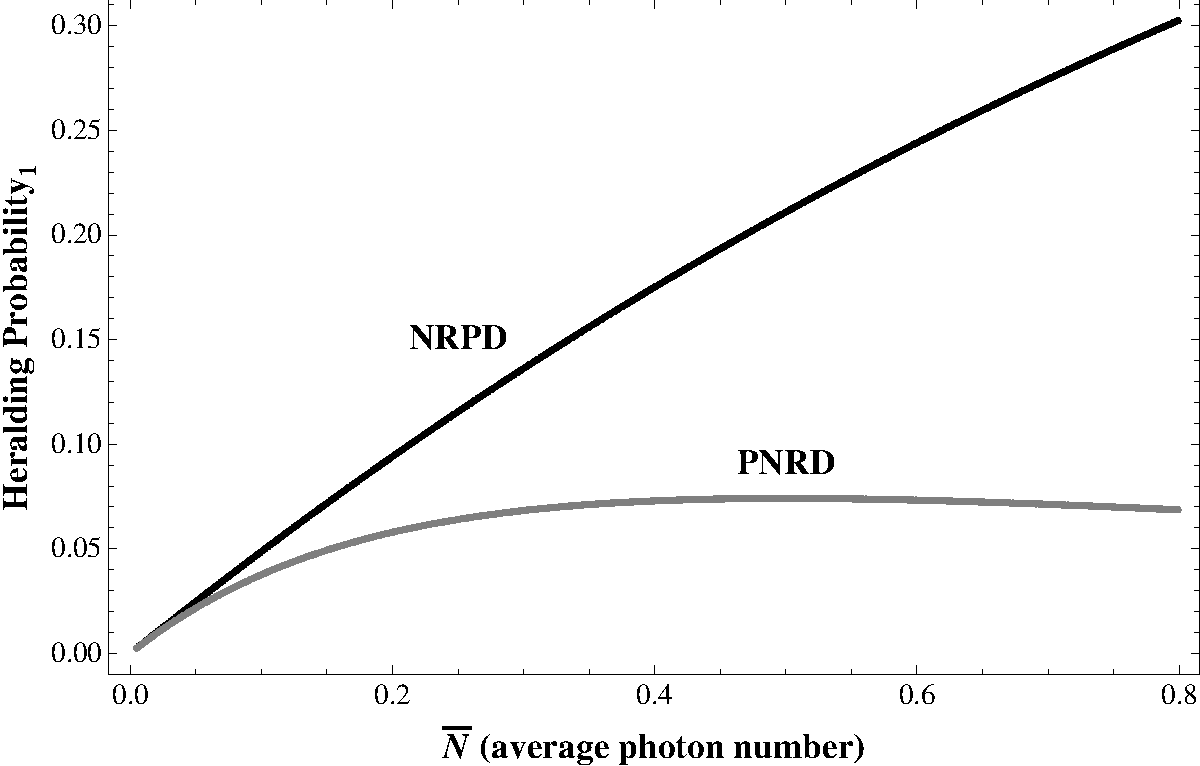
\includegraphics[width=0.47\textwidth]{figures/nrpd_lossless_herald.pdf}
\label{fig:chap3:nrpd_lossless_heralding_prob}
}
\subfigure{
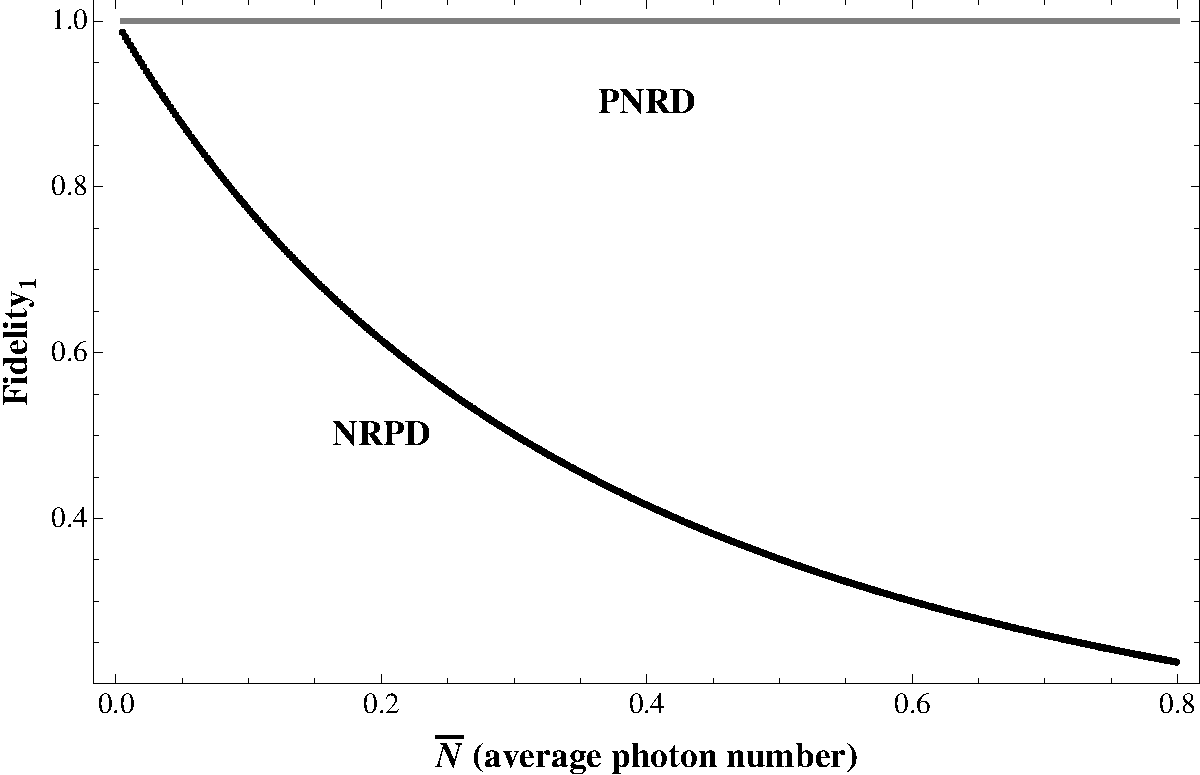
\includegraphics[width=0.47\textwidth]{figures/nrpd_lossless_fid.pdf}
\label{fig:chap3:nrpd_lossless_fidelity}
}
\subfigure{
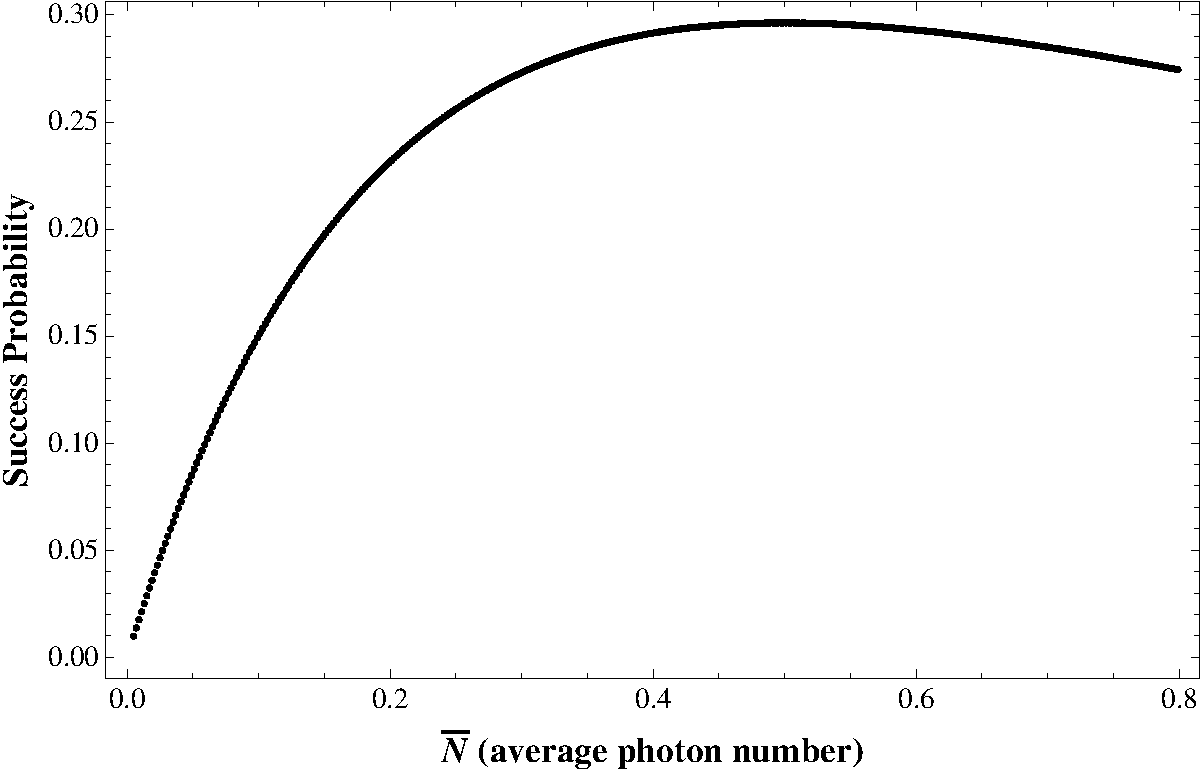
\includegraphics[width=0.47\textwidth]{figures/nrpd_lossless_success.pdf}
\label{fig:chap3:nrpd_lossless_success}
}

\caption{\label{fig:chap3:nrpd_lossless}Figures of merit for lossless architecture (PNRD and NRPD). Figures~\ref{fig:chap3:nrpd_lossless_heralding_prob} and~\ref{fig:chap3:nrpd_lossless_fidelity} show divergences between heralding probability and fidelity for PNRD (gray) and NRPD (black) architectures. The protocol's overall success probability is identical in either case (Fig.~\ref{fig:chap3:nrpd_lossless_success}).}
\end{figure}

Despite the absence of losses in this example, we can still gain some intuition
for the effects of different photodetection schemes on our figures of
merit. Fig.~\ref{fig:chap3:nrpd_lossless} compares the resulting figures of
merit between the PNRD and NRPD photodetection schemes in a lossless
architecture in which increasing $\bar{N}$ leads to an increasing likelihood of
multi-pair emissions from the entanglement source. The heralding probability
for the NRPD exceeds that for PNRD, which is not surprising, as PNRD forms a
subset of the possible detection events present with the NRPD scheme. In the
absence of loss, the NRPD fidelity is independent of detection events at either
$D_{1}/D_{4}$ or $D_{2}/D_{3}$ and falls dramatically for high values of
$\bar{N}$, being ultimately unable to distinguish between valid single-photon
heralding events and higher-order excitations stored in the ensemble. The PNRD
fidelity, on the other hand, holds at unity, because this detector perfectly
identifies single-pair loading in the lossless scenario under consideration
here. The success probability, however, is identical for the PNRD and NRPD
schemes, because any decline in NRPD fidelity is compensated for by a
corresponding increase in heralding probability. A single term in the success
probability sum---the product of the fidelity and heralding
probability---represents the joint probability of loading the required Bell
state and the measurement of the corresponding heralding event. Single photon
events do not require photon-number resolving capabilities, and as such, the
loading success is equally likely under either scheme, when the system is
lossless.

\subsection{Calculation Examples --- Pre-Transmission and Photodetection
  Losses\label{sec:example:two}}

Including loss in our analysis introduces nested binomial distributions of pump
and signal photons, and the added computational complexity of deeper and deeper
nested summations. As such, the results of this example and all subsequent
sections are calculated numerically, with a range of $\bar{N}$ chosen so that
the input Gaussian state can be safely truncated to a finite number of
excitations. For all subsequent calculations in this thesis, $\bar{N}$ ranges
from 0.05 to 0.3 in steps of $\Delta \bar{N}=0.05$, and we take
$n_{\textrm{max}}=m_{\textrm{max}}=3$ to be the maximum number of
excitations. For the the full range of a single transmission efficiency $ 0
\leq \eta \leq 1$, it can be shown (numerically) that figures of merit, such as
heralding probability, with higher truncation values differ insignificantly
from those calculated at $n_{\textrm{max}}=m_{\textrm{max}}=3$. 

Introducing auxiliary vacuum states indexed by $N^{\textrm{pre}}$ and
$N^{\textrm{pho}}$, the joint output state of the heralded photons, ensemble
excitations, and noise modes is given by,
\begin{align}
	\ket{\psi}_{\textrm{out}} &=\sum_{N_i^a,N_i^{\textrm{pre}},N_i,N_i^{\textrm{pho}}}
	\sum_{n,m} 
	f_{n,m}\pna{\bar{N}}
	B_{N_i^a,N_i^{\textrm{pre}}}^{n_i,0}\pna{\eta_i^{\textrm{pre}}}  
	B_{N_2,N_1}^{N_1^a,N_2^a}\pna{\frac{1}{2}}  
	B_{N_4,N_3}^{N_3^a,N_4^a}\pna{\frac{1}{2}}\nonumber \\
	& \qquad \qquad \qquad \qquad \qquad
	\cdot B_{N_i^p,N_i^{\textrm{pho}}}^{N_i,0}\pna{\eta_i^{\textrm{pho}}}  
	\ket{N_i^p}^i_p
	\ket{N_i^a}^i_S 
	\ket{N_i^{\textrm{pre}}}^i_{\textrm{pre}}
	\ket{N_i^{\textrm{pho}}}^i_{\textrm{pho}}. \label{eq:chap3:full_state}
\end{align}
Eqn.~\ref{eq:chap3:full_state} contains several important features. First,
recall that each term indexed by $i$ actually represents four independent
terms. The $n_i$ photons from the SPDC source mix with vacuum (zero photons),
converting into $N^a_i$ pump photons for the quantum memory and
$N_i^{\textrm{pre}}$ noise photons. The pump photons are completely converted
into $N^a_i$ heralding photons and $N^a_i$ spin excitations. At the 50-50 beam
splitter, the $\pna{N^a_1,N^a_2}$ and $\pna{N^a_3,N^a_4}$ photons interfere,
yielding $\pna{N_1,N_2}$ and $\pna{N_3,N_4}$ photons which are each mixed with
vacuum to yield $N^p_i$ photons at each $D_i$ photodetector. The summation
lower limit for each summation variable is 0, and upper limit is given by the
sum of the inputs to a given beam splitter (e.g., $n_i$ for each the $N^a_i$
and $N_i^{\textrm{pre}}$ summations, $N^a_1+N^a_2$ for each of the $N_1$ and
$N_2$ summations). Tracing out the noise modes and and applying photon-number
conservation to eliminate nested summations, the PNRD heralding probability for
single-photon counts at detectors $D_1$ and $D_4$ is given by
\begin{align}
	P_{1}^{\textrm{PNRD}}&=\sum_{N_i^a,N_i}\sum_{n,m}
	\left| f_{n,m}\pna{\bar{N}}
	B_{N_i^a,n_i-N_i^a}^{n_i,0}\pna{\eta_i^{\textrm{pre}}}
	B_{N_2,N_1}^{N_1^a,N_2^a}\pna{\frac{1}{2}}  
	B_{N_4,N_3}^{N_3^a,N_4^a}\pna{\frac{1}{2}} \right. \nonumber \\
	& \qquad \qquad \qquad\left.~\cdot B_{1,N_1-1}^{N_1,0}\pna{\eta_1^{\textrm{pho}}} 
	B_{0,N_2}^{N_2,0}\pna{\eta_2^{\textrm{pho}}} 
	B_{0,N_3}^{N_3,0}\pna{\eta_3^{\textrm{pho}}} 
	B_{1,N_4-1}^{N_4,0}\pna{\eta_4^{\textrm{pho}}} \right|^2. 
\end{align}
From Eqn.~\ref{eqn:coefficient_value}, the photon-number probability amplitude
following the OPA coefficient corresponds to the familiar binomial probability
distribution that results from mixing of a number state with vacuum. Applying
the NRPD POVM and photon-number conservation, as in
Eqn.~\ref{eqn:post:lossless}, and factoring the remaining photodetection
efficiency amplitudes gives the heralding probability:
\begin{align}
	&P_{1}^{\textrm{NRPD}}= \nonumber \\
	& \sum_{N_i^a,N_i}\sum_{n,m}
	\left|f_{n,m}\pna{\bar{N}}
	B_{N_i^a,n_i-N_i^a}^{n_i,0}\pna{\eta_i^{\textrm{pre}}}
	B_{N_2,N_1}^{N_1^a,N_2^a}\pna{\frac{1}{2}}
	B_{N_4,N_3}^{N_3^a,N_4^a}\pna{\frac{1}{2}} 
	B_{0,N_2}^{N_2,0}\pna{\eta_2^{\textrm{pho}}} 
	B_{0,N_3}^{N_3,0}\pna{\eta_3^{\textrm{pho}}}\right|^2\nonumber \\
	&  \pnb{\abs{B_{0,N_1}^{N_1,0}\pna{\eta_1^{\textrm{pho}}}}^2-\sum_{N_1^p=0}^{N_1} \abs{B_{N_1^p,N_1-N_1^p}^{N_1,0}\pna{\eta_1^{\textrm{pho}}}}^2} \pnb{\abs{B_{0,N_4}^{N_4,0}\pna{\eta_4^{\textrm{pho}}}}^2-\sum_{N_4^p=0}^{N_4} \abs{B_{N_4^p,N_4-N_4^p}^{N_4,0}\pna{\eta_4^{\textrm{pho}}}}^2}.
\end{align}
The terms of this summation are also the diagonal coefficients of the
ensembles' post-measurement density operator, which is required for calculating
the fidelity and overall success probability of the protocol. To avoid
redundancy, the numerical calculations of these quantities and their
interpretation is described in Section~\ref{sec:numerics}. 

\subsection{Full Loss Calculation (PNRD and NRPD)~\label{sec:numerics}}

In the previous section, we previewed a set of techniques used in the analysis
of entanglement distribution, which we now use to account for all losses. In
the following, we assume that the input field phase shifts ($\phi_t,\phi_r$) of
each loss-modeling beam splitter are identically 0. As in the previous
sections, we only list expressions for matching photodetection events at $D_1$
and $D_4$, as corresponding expressions for $D_2$ and $D_3$ are found by simple
substitution. Accounting for all losses, the full output state of the
architecture, as shown in Fig.~\ref{fig:channel_loss_model}, is given by,
\begin{align}
\ket{\psi}_{\textrm{out}} & = \sum_{n,m} f_{n,m}\pna{\bar{N}} \nonumber \\
& \hspace{-5mm}\cdot
\sum_{\substack{N_i^a,N_i^{\textrm{pre}},N_i^l,N_i^{\textrm{post}},\\ N_i,N_i^p,N_i^{\textrm{pho}} }}
\pnb{\underbrace{B_{N_i^a,N_i^{\textrm{pre}}}^{n_i,0}\pna{\eta_i^{\textrm{pre}}}  
B_{N_i^l,N_i^{\textrm{post}}}^{N_i^a,0}\pna{\eta_i^{\textrm{post}}}}_\text{Pre-Interference Loss}
\underbrace{B_{N_2,N_1}^{N_1^l,N_2^l}\pna{\frac{1}{2}} B_{N_4,N_3}^{N_3^l,N_4^l}\pna{\frac{1}{2}}}_\text{Interference Terms}
\underbrace{B_{N_i^p,N_i^{\textrm{pho}}}^{N_i,0}\pna{\eta_i^{\textrm{pho}}}}_\text{Photodetection Loss}}   \nonumber \\
& \qquad \quad \cdot \underbrace{\ket{N_i^p}_{p}^i \ket{N_i^a}_{S}^i}_\text{Heralded \& Ensemble Modes} \underbrace{\ket{N_i^{\textrm{pho}}}_{\textrm{pho}}^i \ket{N_i^{\textrm{post}}}_{\textrm{post}}^i \ket{N_i^{\textrm{pre}}}_{\textrm{pre}}^i}_\text{Auxiliary Noise Modes}. 
\end{align}
and the corresponding joint density operator of the heralded photon and
ensemble modes is 
\begin{align}
	\hat{\rho}_{\textrm{out}}^{p,S} & = \sum_{n,m,n',m'} f_{n,m}\pna{\bar{N}} f_{n',m'}\pna{\bar{N}} \nonumber \\
	& \qquad \cdot\sum_{\substack{N_i^a,N_i^{\textrm{pre}}\\ N_i^{a\prime} }} \sum_{\substack{N_i^l,N_i^{\textrm{post}}\\ N_i^{l\prime} }}
	B_{N_i^a,N_i^{\textrm{pre}}}^{n_i,0}\pna{\eta_i^{\textrm{pre}}} B_{N_i^l,N_i^{\textrm{post}}}^{N_i^a,0}\pna{\eta_i^{\textrm{post}}} \pnb{B_{N_i^{a\prime},N_i^{\textrm{pre}}}^{n_i',0}\pna{\eta_i^{\textrm{pre}}} B_{N_i^{l\prime},N_i^{\textrm{post}}}^{N_i^{a\prime},0}\pna{\eta_i^{\textrm{post}}}}^{*} \nonumber \\
	& \qquad \cdot \sum_{\substack{N_1,N_2,N_3,N_4\\ N_1',N_2',N_3',N_4'}}
	 B_{N_2,N_1}^{N_1^l,N_2^l}\pna{\frac{1}{2}} B_{N_4,N_3}^{N_3^l,N_4^l}\pna{\frac{1}{2}} \pnb{B_{N_2',N_1'}^{N_1^{l\prime},N_2^{l\prime}}\pna{\frac{1}{2}} B_{N_4',N_3'}^{N_3^{l\prime},N_4^{l\prime}}\pna{\frac{1}{2}}}^{*}\nonumber \\
	& \qquad \cdot \sum_{\substack{N_i^p,N_i^{\textrm{pho}}\\ N_i^{p\prime} }}
	 B_{N_i^p,N_i^{\textrm{pho}}}^{N_i,0}\pna{\eta_i^{\textrm{pho}}} \pnb{B_{N_i^{p\prime},N_i^{\textrm{pho}}}^{N_i',0}\pna{\eta_i^{\textrm{pho}}}}^{*} \ket{N_i^p}_{p}^i \ket{N_i^a}_{S}^i \bra{N_i^{p\prime}}_{p}^i \bra{N_i^{a\prime}}_{S}^i,
\end{align}
and the PNRD probability that a heralding event $\hat{M}_{1}$ has occurred is then
\begin{align}
	P_{1}& =\textrm{tr}\pna{\hat{\rho}_{\textrm{out}}^{p,S} M_{1}}\nonumber \\
	& = \sum_{n,m}^{\infty} \pnb{f_{n,m}\pna{\bar{N}} }^2 \sum_{N_i^a,N_i^l} \sum_{\substack{N_1,N_2,\\N_3,N_4}} \left|B_{N_i^a,n_i-N_i^a}^{n_i,0}\pna{\eta_i^{\textrm{pre}}}  
	B_{N_i^l,N_i^a-N_i^l}^{N_i^a,0}\pna{\eta_i^{\textrm{post}}}  B_{N_2,N_1}^{N_1^l,N_2^l}\pna{\frac{1}{2}} B_{N_4,N_3}^{N_3^l,N_4^l}\pna{\frac{1}{2}}\right.\nonumber \\
	& \left.\qquad \cdot B_{1,N_1-1}^{N_1,0}\pna{\eta_1^{\textrm{pho}}}
	 		B_{0,N_2}^{N_2,0}\pna{\eta_2^{\textrm{pho}}}
	 		B_{0,N_3}^{N_3,0}\pna{\eta_3^{\textrm{pho}}}
			B_{1,N_4-1}^{N_4,0}\pna{\eta_4^{\textrm{pho}}}\right|^2.
\end{align}

\begin{figure*}[t]
\centering
\subfigure[Single loss ($\eta_1^{\textrm{pre}}$).]{
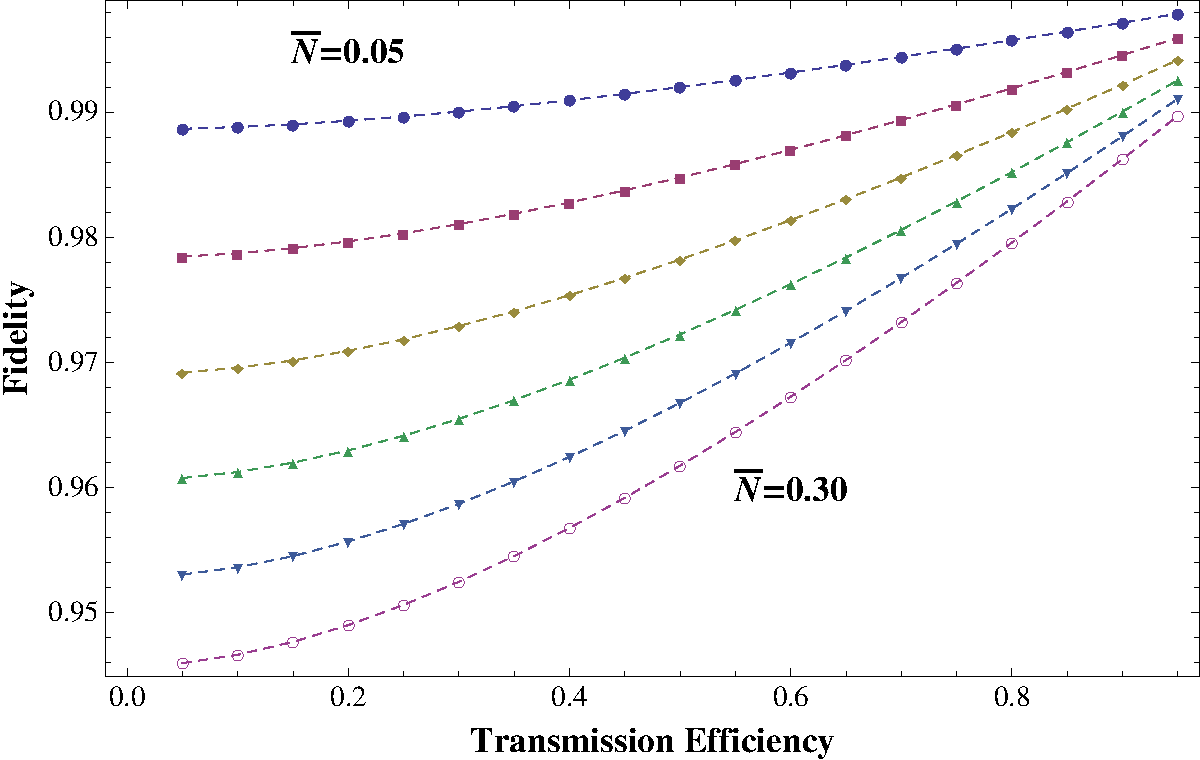
\includegraphics[width=0.47\textwidth]{figures/F14PostSinglePLOT.pdf}
\label{fig:chap3:F14PostSinglePLOT}
}
\subfigure[Signal path losses ($\eta_1^{\textrm{pre}}$ and $\eta_2^{\textrm{pre}}$).]{
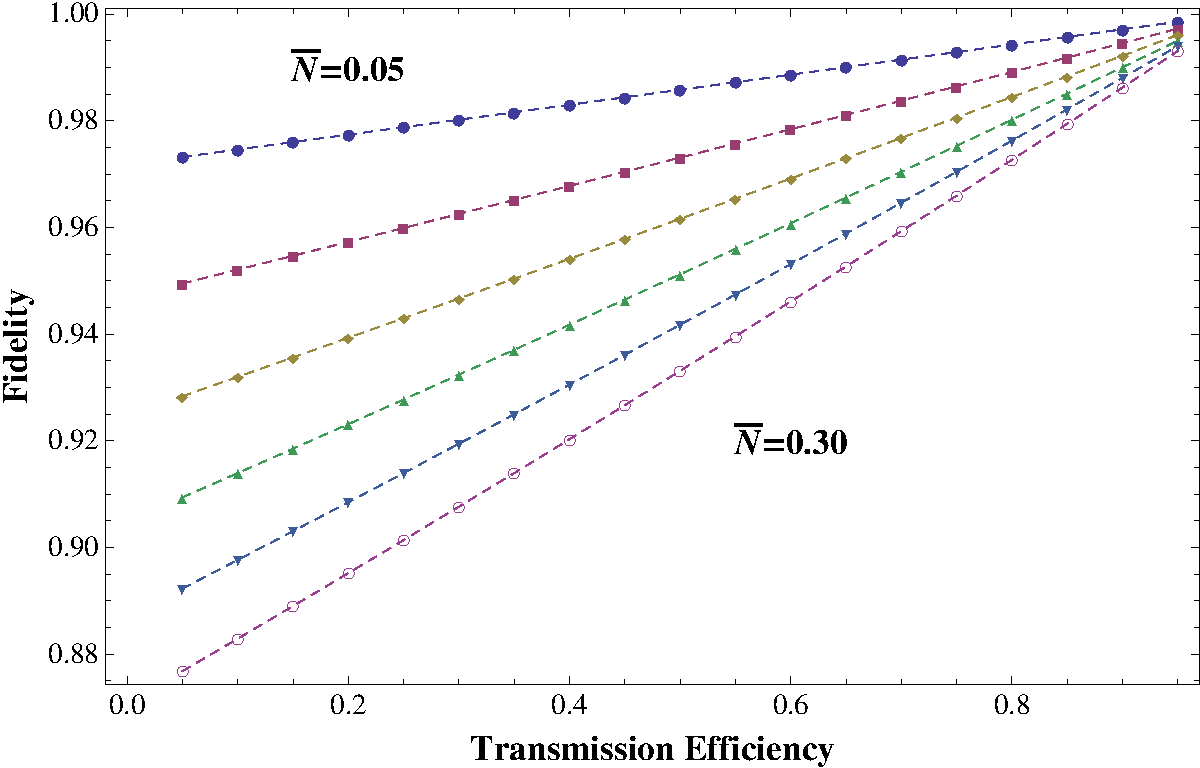
\includegraphics[width=0.47\textwidth]{figures/F14PostMisMatchedPLOT.pdf}
\label{fig:chap3:F14PostMisMatchedPLOT}
}
\subfigure[Mis-matched losses ($\eta_1^{\textrm{pre}}$ and $\eta_3^{\textrm{pre}}$).]{
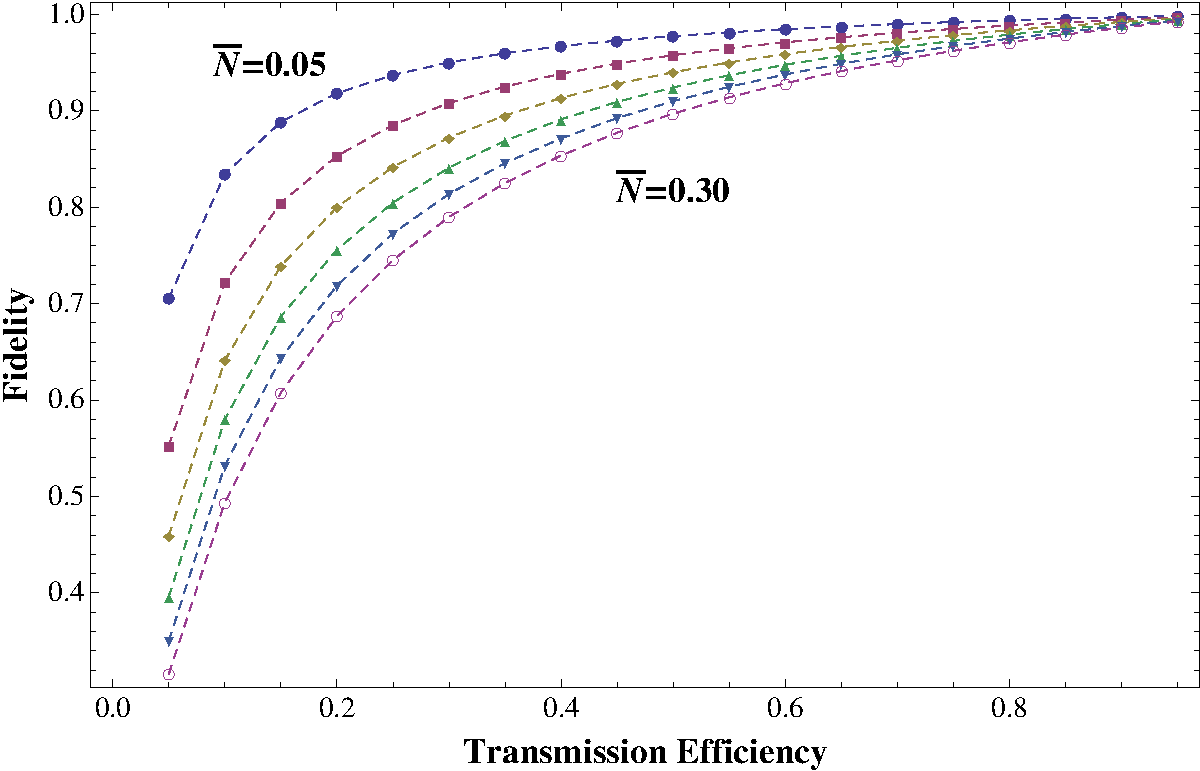
\includegraphics[width=0.47\textwidth]{figures/F14PostMisMatchedCompPLOT.pdf}
\label{fig:chap3:F14PostMisMatchedCompPLOT}
}
\subfigure[Matched losses ($\eta_1^{\textrm{pre}}$ and $\eta_4^{\textrm{pre}}$).]{
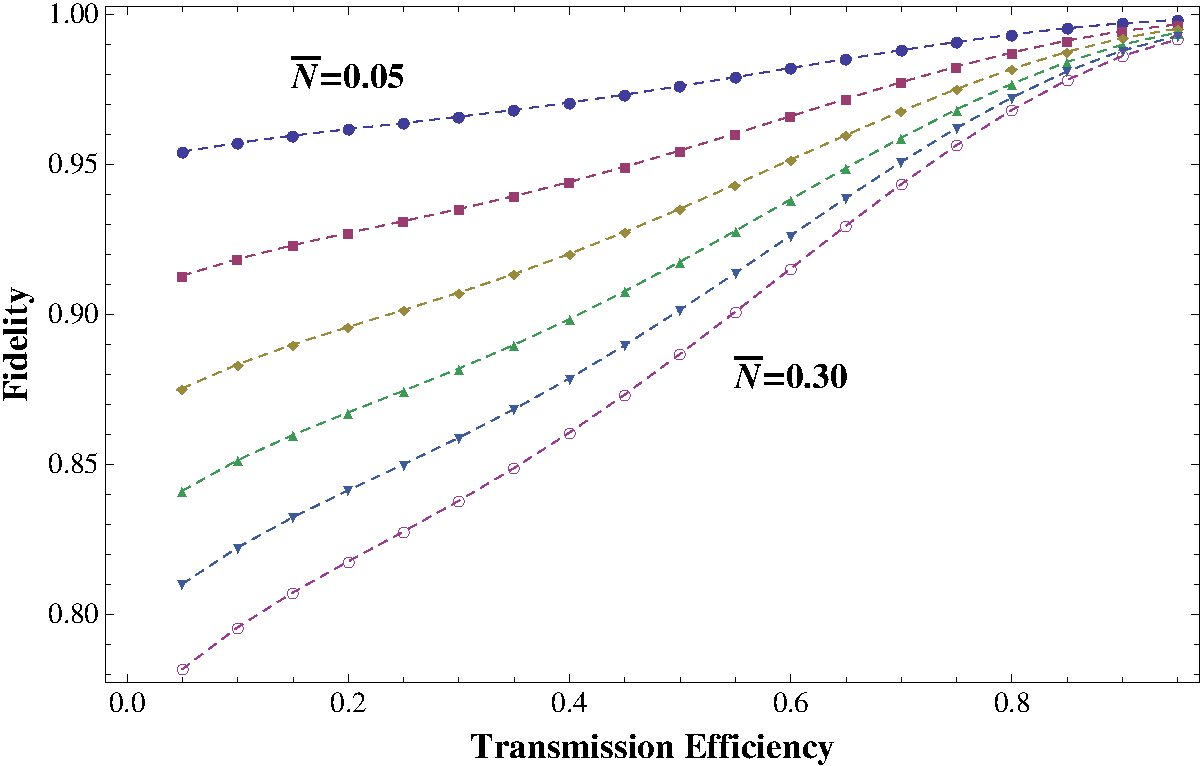
\includegraphics[width=0.47\textwidth]{figures/F14PostMatchedPLOT.pdf}
\label{fig:chap3:F14PostMatchedPLOT}
}
\caption{\label{fig:chap3:asymmetric_pnrd_lossy} $F_1$ fidelities with non-uniform pre-transmission losses (PNRD) for $\bar{N}=0.05-0.3~\pna{\Delta \bar{N}=0.05}$. The caption in each subfigure specifies which of $\eta_i^{\textrm{pre}}~\pna{i=1,2,3,4}$ is varied for that calculation; those not specified are fixed at $0.9$.}
\end{figure*}

\begin{figure}[ht]
\centering
\subfigure[Heralding probability (uniform loss).]{
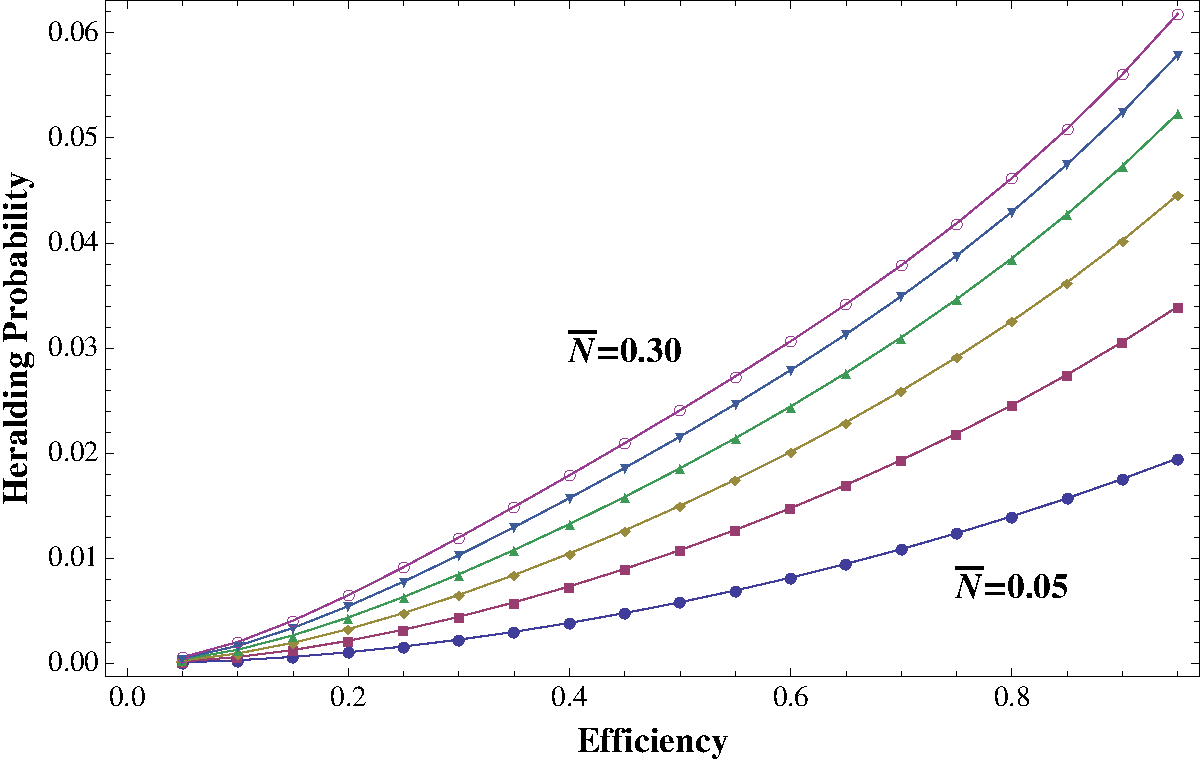
\includegraphics[width=0.47\textwidth]{figures/pnrd_herald_pres.pdf}
\label{fig:chap3:heralding_prob}
}
\subfigure[Fidelity (pre- and photodetection losses).]{
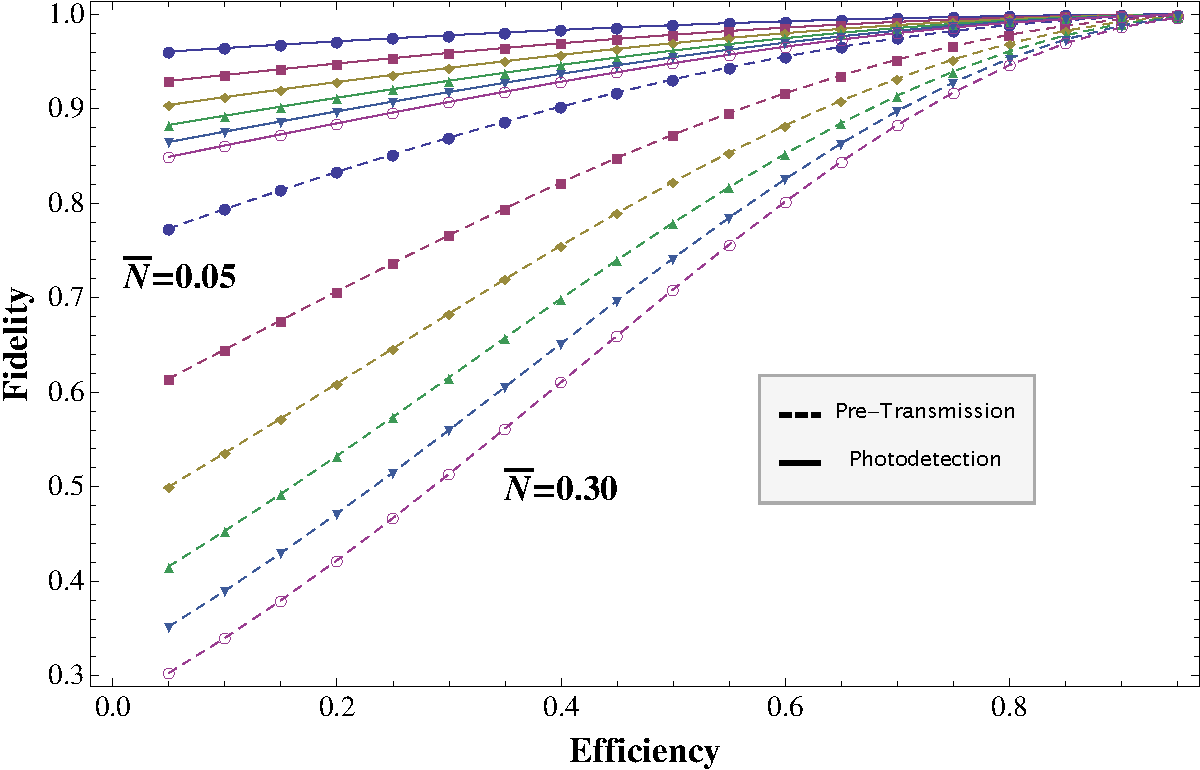
\includegraphics[width=0.47\textwidth]{figures/pnrd_fidelity_pres.pdf}
\label{fig:chap3:fidelity}
}
\caption{\label{fig:chap3:pnrd_data}Figures of merit with uniform losses (PNRD) for $\bar{N}=0.05-0.3~\pna{\Delta\bar{N}=0.05}$. Heralding probabilities are independent of a uniform loss' location: either before (pre-transmission) or after (post-transmission or photodetection) the ensemble (Fig.~\ref{fig:chap3:heralding_prob}). Pre-transmission losses preferentially decrease the fidelity of entanglement distribution compared to post-transmission and photo-detection losses (Fig.~\ref{fig:chap3:fidelity}).}
\end{figure}

The results of numerical calculations with these expressions are shown in
Figures~\ref{fig:chap3:pnrd_data}
and~\ref{fig:chap3:asymmetric_pnrd_lossy}. These figures distinguish between
what we term `uniform' and `non-uniform' losses. Fig.~\ref{fig:chap3:pnrd_data}
assumes that varying pre-transmission and photodetection losses are
\emph{identical} for all four arms of the interferometer, whereas
Fig.~\ref{fig:chap3:asymmetric_pnrd_lossy} makes no such assumption by
considering the effects of only a \emph{single} loss or \emph{paired} losses as
labelled in the captions. The presence of uniform losses in one
location---before or after the ensembles or during photodetections--- has
identical effects on the heralding probability. This heralding probability
doesn't depend on where a single uniform loss is located, as a pump photon lost
prior to the ensemble or a heralding photon lost after the ensemble ultimately
will have the same heralding result. This is definitely not the case for the
$F_1$ fidelity, as a pre-transmission loss of a pump photon precludes
successful entanglement distribution. In this case, it is difficult to tell if
matching signal and idler photons were stored simultaneously. By contrast, any
post-transmission or photodetection loss has a much smaller effect on the
fidelity. Post-transmission and photodetection loss are quantitatively equal in
their fidelity effects. Lastly, increasing pump power in the OPA source matches
intuition, as increasing $\bar{N}$ makes heralding events more likely, but
decreases the desired fidelity due to multiple-pair effects. 

In Fig.~\ref{fig:chap3:asymmetric_pnrd_lossy}, we see that fidelity of
entanglement is fairly robust against a single pre-transmission loss, as well
as uniform losses present only in the signal subsystem or uniform losses
between paths matched for a successful heralding event detection. Uniform
losses shared between mis-matched paths (e.g., varying $\eta_1$ and $\eta_3$)
degrade fidelity significantly, almost as though transmission loss were
uniformly shared by all the paths as in Fig.~\ref{fig:chap3:fidelity}. 

\begin{figure*}[ht]
\centering
\subfigure[$F_1$, uniform pre-transmission loss ($\eta^{\textrm{pre}}$).]{
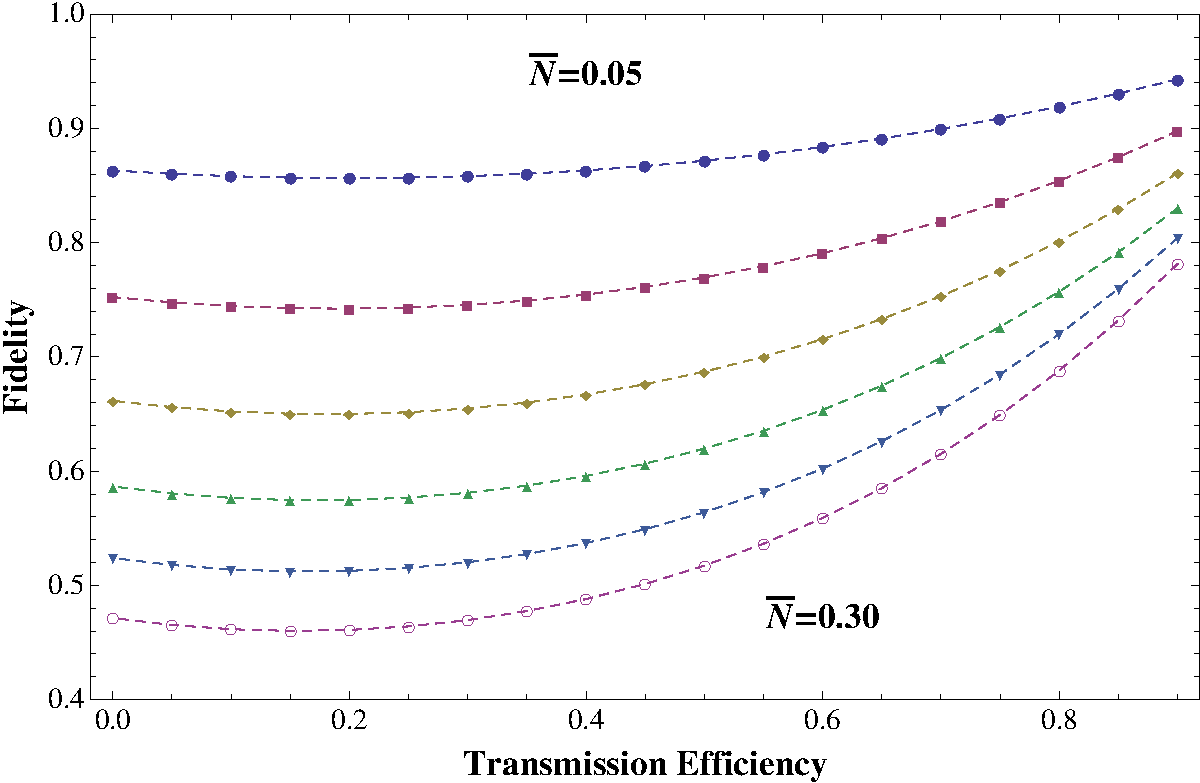
\includegraphics[width=0.47\textwidth]{figures/F14prephoNPRDPreLISTPLOT.pdf}
\label{fig:chap3:F14prephoNPRDPreLISTPLOT}
}
\subfigure[$F_1$, uniform photodetection loss ($\eta^{\textrm{pho}}$).]{
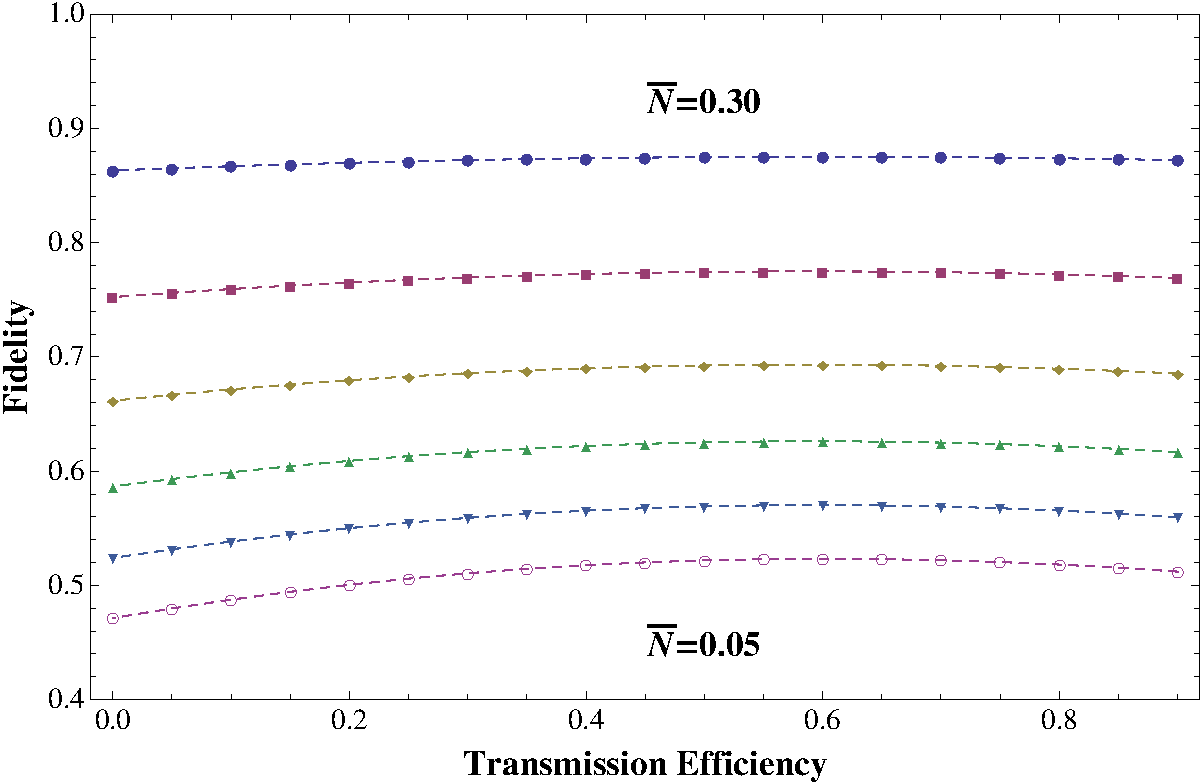
\includegraphics[width=0.47\textwidth]{figures/F14prephoNPRDPhoLISTPlot.pdf}
\label{fig:chap3:F14prephoNPRDPhoLISTPlot}
}
\subfigure[Heralding probability (any uniform loss).]{
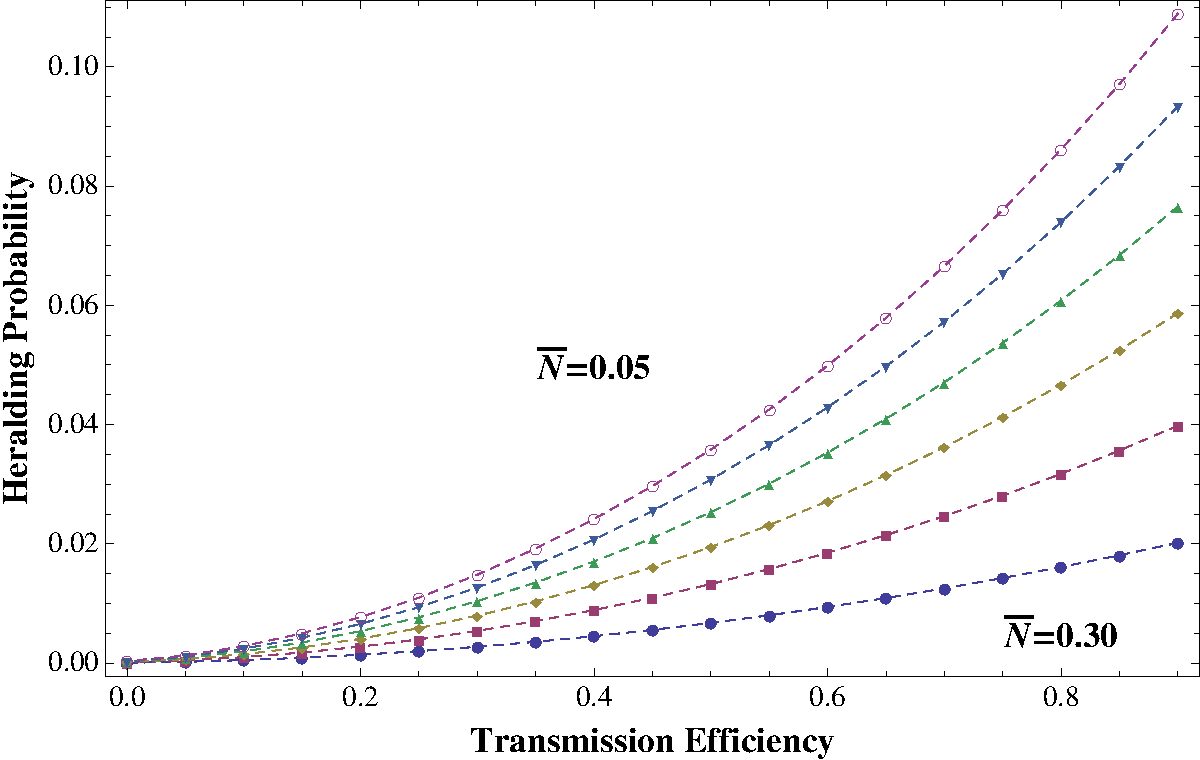
\includegraphics[width=0.47\textwidth]{figures/P14prephoNPRDPhoLIST1PLOT.pdf}
\label{fig:chap3:P14prephoNPRDPhoLIST1PLOT}
}
\caption{\label{fig:chap3:nrpd_lossy} Figures of merit with uniform losses (NRPD) for $\bar{N}=0.05-0.3~\pna{\Delta N = 0.05}$. Figures~\ref{fig:chap3:F14prephoNPRDPreLISTPLOT} and~\ref{fig:chap3:F14prephoNPRDPhoLISTPlot} show the $F_1$ fidelities for varying pre-transmission and photodetection efficiencies, respectively, with all other efficiencies fixed at $\eta=0.9$. Fig.~\ref{fig:chap3:P14prephoNPRDPhoLIST1PLOT} shows heralding probability for varying pre-transmission efficiency.}
\end{figure*}

The remaining analysis case is non-resolving photodetection (NRPD), which we
show in Fig.~\ref{fig:chap3:nrpd_lossy}. The details of this calculation are
nearly identical to that shown in Sections~\ref{sec:example:first}
and~\ref{sec:example:two}. Not surprisingly, as in the lossless NRPD analysis,
the heralding probability is higher than in the PNRD case, and increasing
$\bar{N}$ severely diminishes fidelity when both pre-transmission and
photodetection losses occur. In the case of the latter, photodetection loss has
almost no effect on the final fidelity of entanglement
distribution. Pre-transmission losses in
Fig.~\ref{fig:chap3:F14prephoNPRDPreLISTPLOT} demonstrate a residual dependence
on pre-transmission loss for higher transmission efficiencies, consistent with
our prior PNRD analysis. 


\section{Entanglement Connection~\label{sec:herald:communication}}

\begin{figure*}[htb]
	\centering
	\resizebox{5.00in}{!}{\input ent_connection.pdf_t}
	%\input{spdc_dlcz_fin.pdf_t}
	\caption{Polarization entanglement connection. We assume that ensembles A and B are independently in polarization singlet states or Gaussian states following entanglement distribution in Section~\ref{sec:herald:overview}. The anti-Stokes photons from reading the A and B signal ensembles are interfered at the 50-50 beam splitter. Photon detections at $D_A$ \emph{and} $D_B$ heralds entanglement connection between the idler ensembles A and B.
	\label{fig:entanglement_connection}}
\end{figure*}

After successfully distributing entanglement to a pair of nodes, resulting in
local entanglement, we will want to extend our quantum communication
capabilities over distances prohibited by direct transmission.  In this
section, we use post-selected, polarization-entangled ensembles to accomplish a
basic task in long-distance quantum communication, namely entanglement
swapping. The high level concepts underlying this procedure was described in
Section~\ref{sec:intro:entanglement} of this thesis' introduction, and
is a modification of the DLCZ protocol's application to quantum
communication~\cite{nature35106500}.

Fig.~\ref{fig:entanglement_connection} outlines a procedure for accomplishing
polarization entanglement connection with atomic ensembles. Polarization
entanglement is generated independently, at two different nodes, as described
in Section~\ref{sec:herald:overview} and Fig.~\ref{fig:chap1:connection}. A
Bell-state measurement between the $\pna{S_y^A,S_x^A}$ and $\pna{S_y^B,S_x^B}$
ensemble pairs establishes polarization entanglement between the remaining
idler ensemble pairs $\pna{I_y^A,I_x^A}$ and $\pna{I_y^B,I_x^B}$. Coherent,
on-resonance pulses at each of the signal ensembles reads a Dicke excitation
out of the $\ket{s}-\ket{e}$ atomic transition into a well-defined spatial
mode. Loss-modeling beam splitters before interference ($\eta_{\textrm{pre}}$)
and at photodetection ($\eta_{\textrm{pho}}$) characterize the quantum
efficiency losses, although to maintain consistency with
\cite{PhysRevA.73.042303}, we calculate fidelity with respect to
$\eta_{\textrm{meas}}=\eta_{\textrm{pre}}\eta_{\textrm{pho}}$. In the
following, we determine the fidelity and probability of success when ensembles
A and B are independently in singlet or Gaussian states.

Although a full Bell state measurement is not possible using linear
optics~\cite{PhysRevA.59.3295}, the observation of single clicks at both $D_A$
and $D_B$, when these are unity quantum efficiency photon-number resolving
detectors, uniquely heralds the measurement of a singlet state and successful
completion of entanglement connection protocol when the A and B ensembles were
both in their singlet states. Two signal ensemble pairs in independent singlet
states can be separated into four orthogonal basis states
\begin{align}
& \ket{\psi}^A \otimes \ket{\psi}^B \nonumber \\ 
& \qquad =
\frac{1}{\sqrt{2}}\pna{\ket{1}_{S_y^A}\ket{0}_{S_x^A}\ket{0}_{I_y^A}\ket{1}_{I_x^A}-\ket{0}_{S_y^A}\ket{1}_{S_x^A}\ket{1}_{I_y^A}\ket{0}_{I_x^A}}\nonumber
\\ 
& \qquad \qquad \otimes \frac{1}{\sqrt{2}}\pna{\ket{1}_{S_y^B}\ket{0}_{S_x^B}\ket{0}_{I_y^B}\ket{1}_{I_x^B}-\ket{0}_{S_y^B}\ket{1}_{S_x^B}\ket{1}_{I_y^B}\ket{0}_{I_x^B}} \nonumber \\
& \qquad = \ket{\phi_{yy}}+\ket{\phi_{yx}}+\ket{\phi_{xy}}+\ket{\phi_{xx}},
\end{align}
where each $\ket{\phi_{ij}}~\pna{i,j=x,y}$ labels a joint state with
signal-photon polarizations $i$ and $j$ in each path prior to interference.
Because of photon-twinning at interference, only two of these orthogonal
states---$\ket{\phi_{xy}}$ and $\ket{\phi_{yx}}$---contribute to the
probability of a heralding event: either $\pna{\hat{x},\hat{y}}$- or
$\pna{\hat{y},\hat{x}}$-polarized photon pairs at $\pna{D_A,D_B}$, with equal
probability.  As such, the entanglement connection fidelity will be unity in
both the PNRD and the NPRD cases---
\eqn{
F_C = \frac{P_{\textrm{success}}}{P_{\textrm{herald}}} = \frac{P_{xy}+P_{yx}}{P_{xy}+P_{yx}}=1
}
---independent of pre-transmission and photodetection quantum efficiency losses. 

Now let us consider performance when ensembles A and B are modeled as being in
Gaussian states parameterized by an average spin excitation number
$\bar{N}$. In the absence of any important nonlinear elements in
Fig.~\ref{fig:entanglement_connection}, we will perform a characteristic
function analysis instead of a number-state analysis. The joint density
operator of these ensembles is
$\hat{\rho}_{SI}^{\textrm{in}}=\hat{\rho}_{SI}^A\otimes \hat{\rho}_{SI}^B$,
where $\hat{\rho}_{SI}^i=\hat{\rho}_{S_x^i I_y^i}\otimes\hat{\rho}_{S_y^i
  I_x^i}~\pna{i=A,B}$, which is represented by the anti-normally ordered
characteristic function,
%&=\chi_A^{\rho_{\textrm{in}}^A}\pna{\bm{\zeta}}\chi_A^{\rho_{\textrm{in}}^B}\
% pna{\bm{\zeta}} \nonumber \\
\begin{align}
    \chi_A^{\rho_{\textrm{in}}}\pna{\bm{\zeta}} 
    & =  \langle D_A\pna{\hat{a}_{S_y^A},\zeta_{S_y^A}}
        D_A\pna{\hat{a}_{S_x^A},\zeta_{S_x^A}}
        D_A\pna{\hat{S}_{I_y^A},\zeta_{I_y^A}}
        D_A\pna{\hat{S}_{I_x^A},\zeta_{I_x^A}} \nonumber \\
    & \qquad \cdot D_A\pna{\hat{a}_{S_y^B},\zeta_{S_y^B}}
            D_A\pna{\hat{a}_{S_x^B},\zeta_{S_x^B}}
            D_A\pna{\hat{S}_{I_y^B},\zeta_{I_y^B}}
            D_A\pna{\hat{S}_{I_x^B},\zeta_{S_x^B}}\rangle \nonumber \\
    & = \exp\left[-\pna{1+\bar{N}}\pna{|\zeta_{S_y^A}|^2+|\zeta_{S_x^A}|^2+|\zeta_{I_y^A}|^2+|\zeta_{I_x^A}|^2} \right.\nonumber \\
    & \qquad \qquad \left.{}-\pna{1+\bar{N}}\pna{|\zeta_{S_y^B}|^2+|\zeta_{S_x^B}|^2+|\zeta_{I_y^B}|^2+|\zeta_{I_x^B}|^2}\right.\nonumber \\ 
    & \qquad \qquad \left. {} +2\textrm{Re}\pna{\tilde{N}\zeta_{S_x^A} \zeta_{I_y^A}}-2\textrm{Re}\pna{\tilde{N}\zeta_{S_y^A} \zeta_{I_x^A}}\right.\nonumber \\
    & \qquad \qquad \left. {} +2\textrm{Re}\pna{\tilde{N}\zeta_{S_x^B} \zeta_{I_y^B}}-2\textrm{Re}\pna{\tilde{N}\zeta_{S_y^B} \zeta_{I_x^B}}\right], 
\end{align}
where $\tilde{N}=\sqrt{\bar{N}\pna{\bar{N}+1}}$,
$D_A\pna{\hat{a}_i,\zeta_i}=e^{-\zeta_i^* \hat{a}_i}e^{\zeta_i
  \hat{a}_i^{\dagger}}$ is the antinormally-ordered displacement operator, and
\eqn{
\bm{\zeta} = \pnb{\bm{\zeta}_S, \bm{\zeta}_I}^T= \pnb{\zeta_{S^A_y},\zeta_{S^B_y},\zeta_{S^A_x},\zeta_{S^B_x},
\zeta_{I^A_y},\zeta_{I^B_y},\zeta_{I^A_x},\zeta_{I^B_x}}^{T}.
}
The optical modes reaching the detectors $D_i$ in
Fig.~\ref{fig:channel_loss_model} are
\begin{align}
\mathbf{\hat{a}}^{\textrm{out}}_S & = 
\sqrt{\eta^{\textrm{pho}}\eta^{\textrm{pre}}} \mathbf{B} \mathbf{\hat{a}}^{\textrm{S}}_{\textrm{in}}
+\sqrt{\eta^{\textrm{pho}}\pna{1-\eta^{\textrm{pre}}}}\mathbf{B} \mathbf{\hat{a}}^{\textrm{pre}}_v
 \nonumber \\ & \qquad +\sqrt{1-\eta^{\textrm{pho}}}\mathbf{\hat{a}}^{\textrm{pho}}_v
\end{align}
where we have defined the operator-valued vectors
\begin{align}
	\mathbf{\hat{a}}^{\textrm{out}}_S&=\pnb{\hat{a}_{S^A_y}',\hat{a}_{S^B_y}',\hat{a}_{S^A_x}',\hat{a}_{S^B_x}'}^{\textrm{T}} \nonumber\\
	\mathbf{\hat{a}}_{S}^{\textrm{in}}&=\pnb{\hat{a}_{S^A_y},\hat{a}_{S^B_y},\hat{a}_{S^A_x},\hat{a}_{S^B_x}}^{\textrm{T}} \nonumber\\
	\mathbf{\hat{a}}^{\textrm{pre}}&=\pnb{\hat{a}_1^{\textrm{pre}},\ldots, \hat{a}_4^{\textrm{pre}}}^{\textrm{T}} \nonumber\\
	\mathbf{\hat{a}}^{\textrm{pho}}&=\pnb{\hat{a}^{\textrm{pho}}_1,\ldots, \hat{a}^{\textrm{pho}}_4}^{\textrm{T}}
\end{align}
with the linear transformation of the signal modes:
\eqn{ 
\mathbf{B}=
\left[ 
\begin{array}{cc}
\mathbf{M}_{2\times 2} & \mathbf{0}_{2\times 2} \\
\mathbf{0}_{2\times 2} & \mathbf{M}_{2\times 2}
\end{array} 
\right]
\qquad 
\mathbf{M}_{2\times 2}=
\frac{1}{\sqrt{2}}\left[ 
\begin{array}{cc}
1 & 1 \\
1 & -1\end{array} \right].\label{eqn:chap3:linear_beamsplitter}}
All of the idler modes
$\mathbf{\hat{S}}_{{I}}^{\textrm{in}}=\pnb{\hat{S}_{I^A_y},\hat{S}_{I^B_y},\hat{S}_{I^A_x},\hat{S}_{I^B_x}}^{\textrm{T}}$
remain unchanged. The Gaussian mixed-state of the Stokes light arriving at the
detectors and the idler ensemble excitations is given by the
antinormally-ordered characteristic function
\begin{align}
	& \chi_A^{\rho_{\textrm{out}}}\pna{\bm{\zeta}, \bm{\tilde{\zeta}}}
        \nonumber \\
	& \qquad =\langle D_A\pna{\mathbf{\hat{a}}_S^{\textrm{out}}, \bm{\zeta}_S} D_A\pna{\mathbf{\hat{S}}_I^{\textrm{in}}, \bm{\zeta}_I} \rangle\nonumber \\
	& \qquad = \chi_A^{\rho_{\textrm{in}}}\pna{\pnb{\sqrt{\eta_{\textrm{meas}}}\tilde{\zeta}_{S^A_y},\sqrt{\eta_{\textrm{meas}}}\tilde{\zeta}_{S^B_y},\sqrt{\eta_{\textrm{meas}}}\tilde{\zeta}_{S^A_x},\sqrt{\eta_{\textrm{meas}}}\tilde{\zeta}_{S^B_x},
    \zeta_{I^A_y},\zeta_{I^B_y},\zeta_{I^A_x},\zeta_{I^B_x}}^{T}} \nonumber \\
    & \qquad \qquad \cdot \exp\pnb{-\sum_{\{\tilde{\zeta}_i\}}\eta^{\textrm{pho}}\pna{1- \eta^{\textrm{pre}}}|\tilde{\zeta}_i|^2-\sum_{\{{\zeta}_i\}}\pna{1-\eta^{\textrm{pho}}}|{\zeta}_i|^2} \label{eqn:chap3:chia_orig}
\end{align}
where the scaled $\tilde{\bm{\zeta}}$ result from the transformation of the
beam splitter transformation in Eqn.~\ref{eqn:chap3:linear_beamsplitter}:
\eqn{
\tilde{\bm{\zeta}}=\mathbf{B}^{\dagger}\bm{\zeta}=\left[
\begin{array}{c}
	\tilde{\zeta}_{S_y^A} \\
	\tilde{\zeta}_{S_y^B} \\
	\tilde{\zeta}_{S_x^A} \\
	\tilde{\zeta}_{S_x^B}
\end{array}
\right]=\frac{1}{\sqrt{2}}
\left[
\begin{array}{c}
	\zeta_{S_y^A} + \zeta_{S_y^B} \\
	\zeta_{S_y^A} - \zeta_{S_y^B} \\
	\zeta_{S_x^A} + \zeta_{S_x^B}\\
	\zeta_{S_x^A} - \zeta_{S_x^B}
\end{array}
\right].\label{eq:scaled_vars}
}
Rewriting Eqn.~\ref{eqn:chap3:chia_orig} in terms of $\bm{\zeta}$, the
characteristic function is now
\begin{align}
    \chi_A^{\rho_{\textrm{out}}}\pna{\bm{\zeta}} 
    & = \exp\left[-\pna{1+\eta_{\textrm{meas}}\bar{N}}\pna{|\zeta_{S_y^A}|^2+|\zeta_{S_x^A}|^2+|\zeta_{S_y^B}|^2+|\zeta_{S_x^B}|^2} \right.\nonumber \\
    & \qquad \qquad \left.{}-\pna{1+\bar{N}}\pna{|\zeta_{I_y^A}|^2+|\zeta_{I_x^A}|^2+|\zeta_{I_y^B}|^2+|\zeta_{I_x^B}|^2}\right.\nonumber \\ 
    & \qquad \qquad \left. {} +\tilde{N}\sqrt{2\eta_{\textrm{meas}}}\left[
    \textrm{Re}\pna{\zeta_{S_x^A} \zeta_{I_y^A}}
    +\textrm{Re}\pna{\zeta_{S_x^B}\zeta_{I_y^A}}
    -\textrm{Re}\pna{\zeta_{S_y^A}\zeta_{I_x^A}}
    -\textrm{Re}\pna{\zeta_{S_y^B} \zeta_{I_x^A}}\right.\right.\nonumber \\
    & \qquad \qquad \left.\left. {} 
    +\textrm{Re}\pna{\zeta_{S_x^A}\zeta_{I_y^B}}
    -\textrm{Re}\pna{\zeta_{S_x^B}\zeta_{I_y^B}}
    -\textrm{Re}\pna{\zeta_{S_y^A}\zeta_{I_x^B}}
    +\textrm{Re}\pna{\zeta_{S_y^B} \zeta_{I_x^B}}\right]\right].
    \label{eq:char_final}
\end{align}

A useful property of Gaussian antinormally-ordered characteristic functions is
that they can be renormalized into a probability density function, whose
moments can be calculated. We find the heralding probability and fidelity by
re-expressing Eqn.~\ref{eq:char_final} as
\eqn{
\chi_A^{\rho_{\textrm{out}}}\pna{\bm{\zeta}}=\frac{\pi^8 p_{\mathbf{Z}}\pna{\bm{\zeta}}}{D_1}
}
where $p_{\mathbf{Z}}\pna{\bm{\zeta}}$ is the probability density function for
a zero-mean Gaussian random vector $\bm{\zeta}$ with covariance matrices
\begin{align}
\langle \bm{\zeta}\bm{\zeta}^{\dagger}\rangle&=\frac{1}{D_1}\left[ 
\begin{array}{cc}
\pna{1+\eta_{\textrm{meas}} \bar{N}} \mathbf{I}_{4\times 4} &  \mathbf{0}_{4\times 4} \\
 \mathbf{0}_{4\times 4} & \pna{1+\bar{N}} \mathbf{I}_{4\times 4}
\end{array} 
\right] \nonumber \\
\langle \bm{\zeta}\bm{\zeta}^{T}\rangle&=\frac{1}{D_1}\left[ 
\begin{array}{cc}
 \mathbf{0}_{4\times 4} & \mathbf{N}_{4\times 4} \\
 \mathbf{N}_{4\times 4}^T & \mathbf{0}_{4\times 4}
\end{array} 
\right]\label{eq:chap3:moments}
\end{align}
for 
\eqn{
\mathbf{N}_{4\times 4}=\tilde{N}\sqrt{2\eta_{\textrm{meas}}}\left[ 
\begin{array}{cccc}
0 & 0 & -1 & -1\\
0 & 0 & -1 & 1\\
1 & 1 & 0 & 0\\
1 & -1 & 0 & 0
\end{array} 
\right]
}
and determinant $D_1=\pna{1+\eta_{\textrm{meas}} \bar{N}}^4
\pna{1+\bar{N}}^4-256 \tilde{N}^8 \eta_{\textrm{meas}}^4$. The output density
operator of the Stokes field can be expressed as the operator-valued Fourier
transformation of Eqn.~\ref{eq:char_final}:
\begin{align}
\hat{\rho}_{\textrm{out}}& =\int 
\prod_{i=x,y}
\frac{d^2 \zeta_{I_i^A}}{\pi^2} 
\frac{d^2 \zeta_{I_i^B}}{\pi^2} 
D_N\pna{\hat{S}_{I_i^A},\zeta_{I_i^A}} 
D_N\pna{\hat{S}_{I_i^B},\zeta_{I_i^B}}  \nonumber \\
& \qquad \cdot \int 
\prod_{i=x,y}
\frac{d^2 \zeta_{S_i^A}}{\pi^2} 
\frac{d^2 \zeta_{S_i^B}}{\pi^2}
\chi_A^{\rho_{\textrm{out}}}\pna{\bm{\zeta}} 
D_N\pna{\hat{a}_{S_i^A}',\zeta_{S_i^A}} 
D_N\pna{\hat{a}_{S_i^B}',\zeta_{S_i^B}},
\label{eq:fourier_char}
\end{align}
where $D_N\pna{\hat{a}_i,\zeta_i}=e^{-\zeta_i \hat{a}_i^{\dagger}}e^{\zeta_i^*
  \hat{a}_i}$ is the normally-ordered displacement operator. To perform trace
operations on the operator-valued Fourier transform in
Eqn.~\ref{eq:fourier_char}, we know that
\eqn{
\bra{0} D_N\pna{\hat{a}_i,\zeta_i} \ket{0}=1 \qquad  \bra{1}D_N\pna{\hat{a}_i,\zeta_i}\ket{1}=1-|\zeta_i|^2
}
and that
\begin{align}
\textrm{tr}\pnb{D_N\pna{\hat{a}_i,\zeta_i}} &=\pi\delta\pna{\zeta_i} \nonumber
\\ \textrm{tr}\pnb{D_N\pna{\hat{a}_i,\zeta_i}\pna{\hat{I}-\ket{0}\bra{0}}} &=
\pi\delta\pna{\zeta_i}-1.\label{eq:chap3:trace_id}
\end{align}
Performing trace operations on the $\hat{a}_i$ mode of an output density
operator is equivalent to setting $\zeta_i=0$ in its characteristic function,
so any Gaussian moment calculations in the following may involve a marginal
distribution of that specified by Eqn.~\ref{eq:chap3:moments}.

\begin{figure}[tb]
	\centering
	\centering
    \subfigure[Heralding probability.]{
    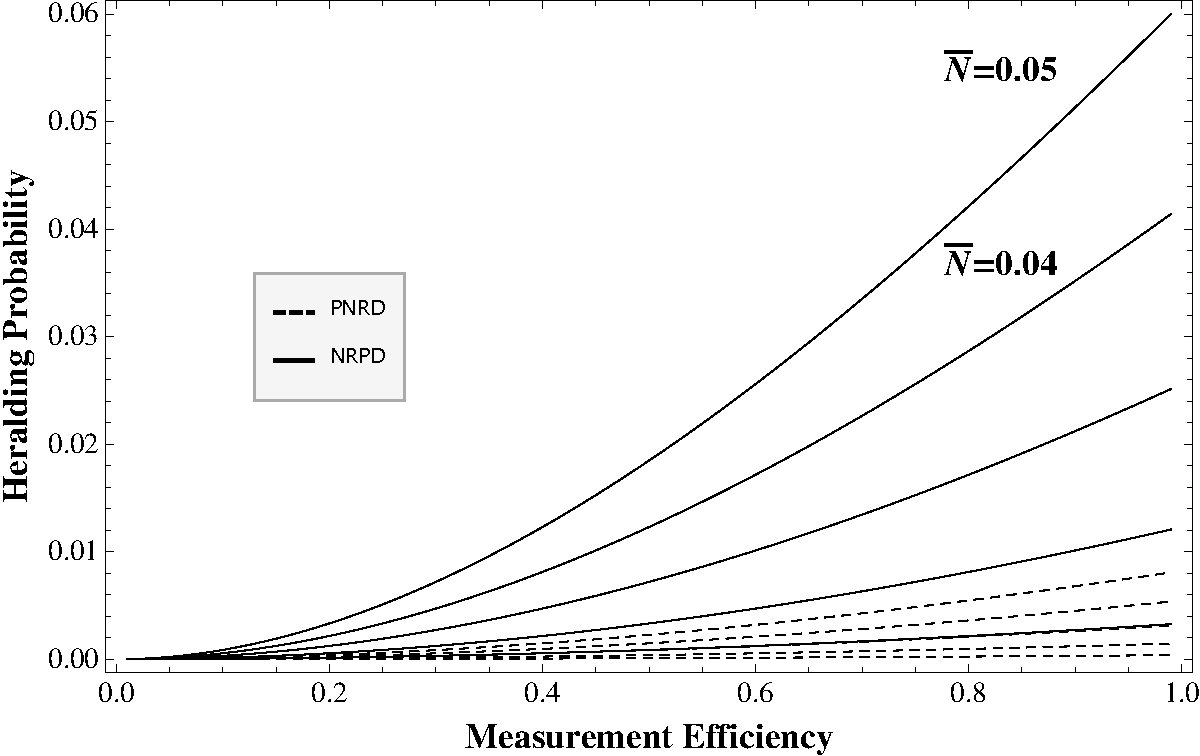
\includegraphics[width=0.47\textwidth]{figures/finalHeraldBothCON.pdf}
    \label{fig:chap3:con:heralding_prob}
    }
    \subfigure[Fidelity of entanglement.]{
    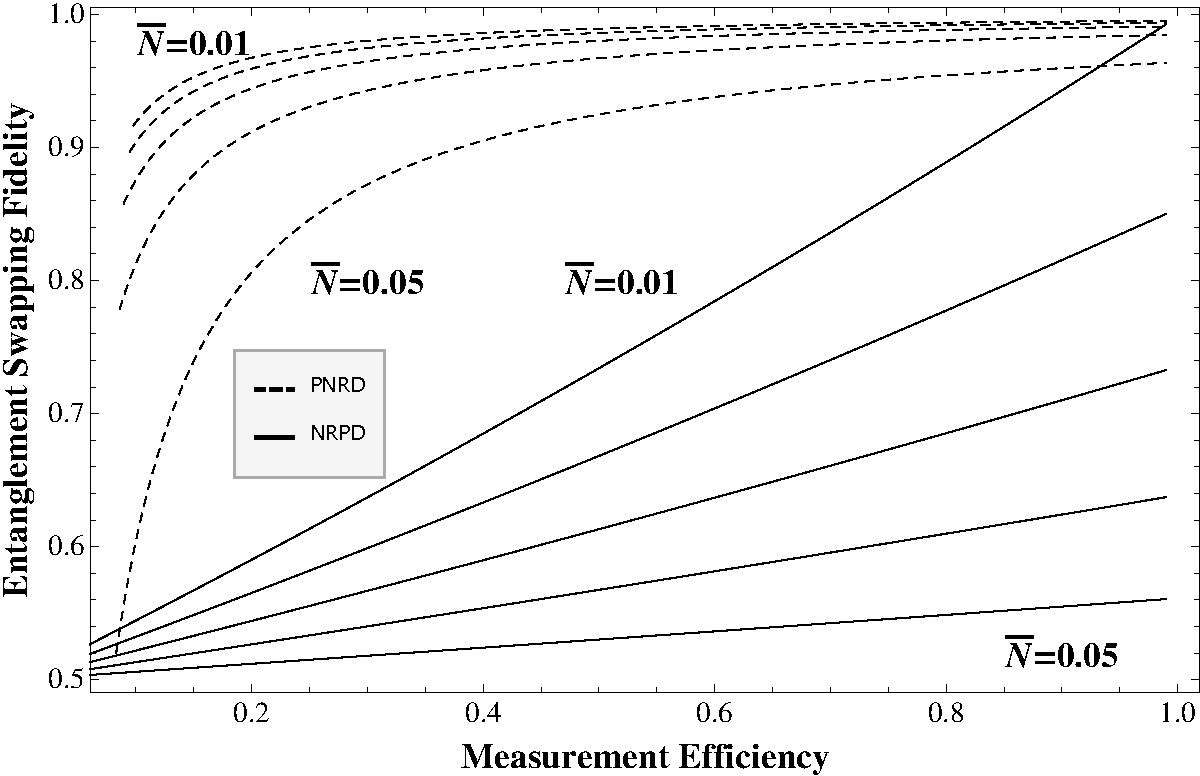
\includegraphics[width=0.47\textwidth]{figures/finalFidelityBothCON.pdf}
    \label{fig:chap3:con:fidelity}
    }
    \subfigure[Fidelity ratio for cross- and co-polarized heralding events.]{
    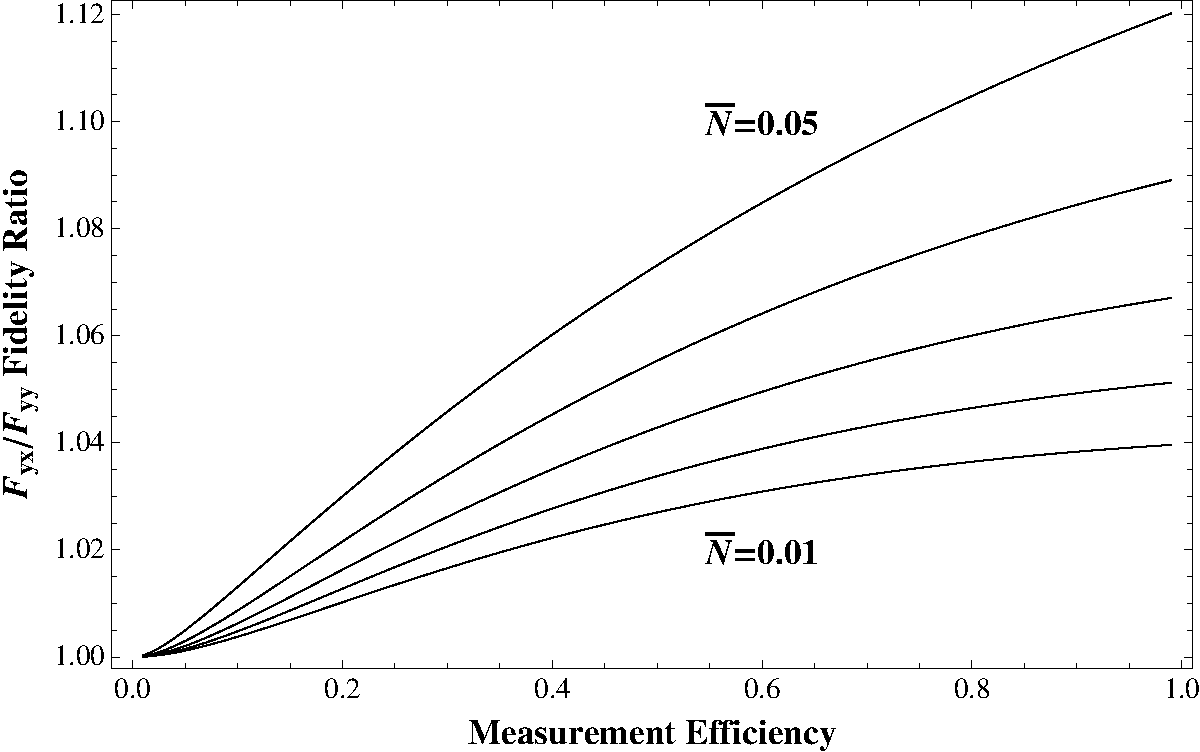
\includegraphics[width=0.47\textwidth]{figures/ratioplot.pdf}
    \label{fig:chap3:con:ratio}
    }
	%\input{spdc_dlcz_fin.pdf_t}
	\caption{Figures of merit for Gaussian state entanglement connection (PNRD and NRPD) for $\bar{N}=0.01-0.05~\pna{\Delta N=0.01}$. 
	\label{fig:merit:entanglement_connection}}
\end{figure}

We will first consider the particular case of a $\mathbf{y}-$polarized click at
$D_A$ and a $\mathbf{x}-$polarized click at $D_B$, and then extrapolate to
other possibilities: a $\mathbf{x}-$polarized click at $D_A$ and a
$\mathbf{y}-$polarized click at $D_B$, and co-polarized clicks at both $D_A$
and $D_B$. Applying these trace identities in a PNRD scheme, the
post-measurement state of the ensembles is
\begin{align}
\hat{\rho}_{\textrm{post}}^{yx}& =
\frac{1}{P_{\textrm{herald}}^{yx}}\int 
\prod_{i=x,y}
\frac{d^2 \zeta_{I_i^A}}{\pi^2} 
\frac{d^2 \zeta_{I_i^B}}{\pi^2} 
D_N\pna{\hat{S}_{I_i^A},\zeta_{I_i^A}} 
D_N\pna{\hat{S}_{I_i^B},\zeta_{I_i^B}}  \nonumber \\
& \qquad \cdot \int 
\frac{d^2 \zeta_{S_y^A}}{\pi^2} 
\frac{d^2 \zeta_{S_x^B}}{\pi^2}
\chi_A^{\rho_{\textrm{out}}}\pna{\bm{\zeta}} 
\pna{1-|\zeta_{S_y^A}|^2}\pna{1-|\zeta_{S_x^B}|^2},
\end{align}
where the heralding probability is
\begin{align}
P_{\textrm{herald}}^{yx} & =
\int 
\frac{d^2 \zeta_{S_y^A}}{\pi^2} 
\frac{d^2 \zeta_{S_x^B}}{\pi^2} \nonumber \\ 
& \qquad \cdot
\chi_A^{\rho_{\textrm{out}}}\pna{\pnb{\zeta_{S_y^A},\zeta_{S_y^B},\zeta_{S_x^A},\zeta_{S_x^B},0,0,0,0}^T}
\nonumber \\ 
& \qquad \cdot \pna{1-|\zeta_{S_y^A}|^2}\pna{1-|\zeta_{S_x^B}|^2}.
\end{align}
Applying the Gaussian moment factoring theorem, this heralding probability is
\begin{align}
P_{\textrm{herald}}^{yx}&=\frac{1}{D_2}\langle \pna{1-|\zeta_{S_y^A}|^2}\pna{1-|\zeta_{S_x^B}|^2} \rangle \nonumber \\
	&=\frac{1}{D_2^3}\pnb{D_2^2-2\pna{1+\eta_{\textrm{meas}}\bar{N}}D_2+\pna{1+\eta_{\textrm{meas}}\bar{N}}^2} \nonumber \\
	& = \frac{\eta^2_{\textrm{meas}} \bar{N}^2 (\eta_{\textrm{meas}}  \bar{N} (\eta_{\textrm{meas}}  \bar{N}+3)+3)^2}{(\eta_{\textrm{meas}}  \bar{N}+1)^{10}},
\end{align}
where $\langle~~\rangle$ denotes ensemble averaging treating $\bm{\zeta}$ as a
complex-valued Gaussian random vector whose probability density function is a
marginal distribution of Eqn.~\ref{eq:chap3:moments}, with
$D_2=\pna{1+\eta_{\textrm{meas}}\bar{N}}^4$. Note that the second-moments of
the signal modes reaching the photodetectors are all identical, so the
heralding probabilities for each of the four heralding probabilities mentioned
earlier are equal. Therefore, $P_{\textrm{herald}}=4P_{\textrm{herald}}^{yx}$
for the PNRD case. Applying the trace identities in
Eqn~\ref{eq:chap3:trace_id}, the post-measurement joint density operator for
the NRPD scheme is
\begin{align}
\hat{\rho}_{\textrm{post}}^{yx}& =
\frac{1}{P_{\textrm{herald}}^{yx}}\int \prod_{i=x,y}
\frac{d^2 \zeta_{I_i^A}}{\pi^2} 
\frac{d^2 \zeta_{I_i^B}}{\pi^2} 
D_N\pna{\hat{S}_{I_i^A},\zeta_{I_i^A}} 
D_N\pna{\hat{S}_{I_i^B},\zeta_{I_i^B}}  \nonumber \\
& \qquad \cdot \int 
\frac{d^2 \zeta_{S_y^A}}{\pi^2} 
\frac{d^2 \zeta_{S_x^B}}{\pi^2}
\chi_A^{\rho_{\textrm{out}}}\pna{\bm{\zeta}} 
\pnb{\pi\delta\pna{\zeta_{S_y^A}}-1}\pnb{\pi\delta\pna{\zeta_{S_x^B}}-1}.
\end{align}
Tracing out the idler excitation modes, the NRPD heralding probability is 
\begin{align}
& P_{\textrm{herald}}^{yx} = \nonumber \ \int 
\prod_{i=x,y}
\frac{d^2 \zeta_{S_i^A}}{\pi^2} 
\frac{d^2 \zeta_{S_i^B}}{\pi^2} \nonumber \\ 
& \qquad \qquad \cdot
\chi_A^{\rho_{\textrm{out}}}\pna{\pnb{\zeta_{S_y^A},\zeta_{S_y^B},\zeta_{S_x^A},\zeta_{S_x^B},0,0,0,0}^T}
\nonumber \\
& \qquad \qquad \cdot 
\pnb{\pi\delta\pna{\zeta_{S_y^A}}-1}\pnb{\pi\delta\pna{\zeta_{S_x^B}}-1},
\end{align}
which yields
\eqn{
P_{\textrm{herald}}^{yx} = \frac{\eta ^2_{\textrm{meas}} \bar{N}^2}{(\eta_{\textrm{meas}}  \bar{N}+1)^4}.
}
This PNRD heralding probability and PNRD fidelity, as well as the NRPD
heralding probability and fidelity are shown in
Fig.~\ref{fig:merit:entanglement_connection}. The results for heralding
probability are consistent with our understanding of multiple-excitation
effects, as described previously in the context of entanglement distribution in
Section~\ref{sec:numerics}: reading from ensembles with a higher average spin
excitation $\bar{N}$ will yield more anti-Stokes photons, resulting in a higher
likelihood of a heralding event when the photodetectors cannot resolve photon
number.

\begin{comment}
The necessary higher-order moments for this calculation are, from Gaussian
moment factoring
\begin{align}
 \langle |\zeta_{I_x^A}\zeta_{I_y^B}-\zeta_{I_y^A}\zeta_{I_x^B}|^2 \rangle & = \langle |\zeta_{I_x^A}|^2 \rangle \langle |\zeta_{I_y^B}|^2 \rangle+\langle |\zeta_{I_y^A}|^2 \rangle \langle |\zeta_{I_x^B}|^2\rangle \nonumber \\
 \langle |\zeta_{S_y^A}|^2  |\zeta_{I_x^A}\zeta_{I_y^B}-\zeta_{I_y^A}\zeta_{I_x^B}|^2 \rangle & = \langle |\zeta_{S_y^A}|^2\rangle \langle |\zeta_{I_x^A}|^2\rangle \langle |\zeta_{I_y^B}|^2\rangle + \langle |\zeta_{S_y^A}|^2\rangle \langle |\zeta_{I_y^A}|^2\rangle \langle |\zeta_{I_x^B}|^2\rangle \nonumber \\
 & \qquad + |\langle \zeta_{S_y^A} \zeta_{I_x^A}\rangle|^2 \langle | \zeta_{I_y^B} |^2\rangle + |\langle \zeta_{S_y^A} \zeta_{I_x^B} \rangle|^2 \langle | \zeta_{I_y^A}  |^2\rangle \nonumber \\
 \langle |\zeta_{S_x^B}|^2 |\zeta_{I_x^A}\zeta_{I_y^B}-\zeta_{I_y^A}\zeta_{I_x^B}|^2 \rangle & = \langle |\zeta_{S_x^B}|^2\rangle \langle |\zeta_{I_x^A}|^2\rangle \langle |\zeta_{I_y^B}|^2\rangle + \langle |\zeta_{S_x^B}|^2\rangle \langle |\zeta_{I_y^A}|^2\rangle \langle |\zeta_{I_x^B}|^2\rangle \nonumber \\
  & \qquad + |\langle \zeta_{S_x^B} \zeta_{I_y^B}\rangle|^2 \langle | \zeta_{I_x^A} |^2\rangle + |\langle \zeta_{S_x^B} \zeta_{I_y^A} \rangle|^2 \langle | \zeta_{I_x^B}  |^2\rangle \nonumber \\
 \langle |\zeta_{S_y^A}|^2  |\zeta_{S_x^B}|^2 |\zeta_{I_x^A}\zeta_{I_y^B}-\zeta_{I_y^A}\zeta_{I_x^B}|^2 \rangle  & = \langle |\zeta_{S_y^A}|^2\rangle \langle |\zeta_{S_x^B}|^2\rangle \langle |\zeta_{I_x^A}|^2\rangle \langle |\zeta_{I_y^B}|^2\rangle \nonumber \\
 & + \langle |\zeta_{S_y^A}|^2\rangle \langle |\zeta_{S_x^B}|^2\rangle \langle |\zeta_{I_y^A}|^2\rangle \langle |\zeta_{I_x^B}|^2\rangle \nonumber \\
   &  + |\langle \zeta_{S_y^A} \zeta_{I_x^A}\rangle|^2 |\langle \zeta_{S_x^B} \zeta_{I_y^B}\rangle|^2+ |\langle \zeta_{S_y^A} \zeta_{I_x^B} \rangle|^2 |\langle \zeta_{S_x^B} \zeta_{I_y^A} \rangle|^2  \nonumber \\
   &  + |\langle \zeta_{S_y^B} \zeta_{I_x^A}\rangle|^2 \langle| \zeta_{S_x^B}|^2\rangle \langle|\zeta_{I_y^B}|^2\rangle + |\langle \zeta_{S_y^A} \zeta_{I_x^B}\rangle|^2 \langle| \zeta_{S_x^B}|^2\rangle \langle|\zeta_{I_y^B}|^2\rangle  \nonumber \\
     &  + |\langle \zeta_{S_x^B} \zeta_{I_y^B}\rangle|^2 \langle| \zeta_{I_x^A}|^2\rangle \langle|\zeta_{S_y^A}|^2\rangle + |\langle \zeta_{S_x^B} \zeta_{I_y^A}\rangle|^2 \langle| \zeta_{S_y^A}|^2\rangle \langle|\zeta_{I_x^B}|^2\rangle \nonumber \\
     &-\left[\langle \zeta_{S_y^A} \zeta_{I_x^A}\rangle \langle \zeta_{S_y^{A}}^* \zeta_{I_x^{B}}^*\rangle \langle \zeta_{S_x^B} \zeta_{I_y^B}\rangle \langle \zeta_{S_x^{B}}^* \zeta_{I_y^{A}}^*\rangle \right.\nonumber \\
     & \left.\qquad\qquad + \langle \zeta_{S_y^A} \zeta_{I_x^B}\rangle \langle \zeta_{S_y^{A}}^* \zeta_{I_x^{A}}^*\rangle \langle \zeta_{S_x^B} \zeta_{I_y^A}\rangle \langle \zeta_{S_x^{B}}^* \zeta_{I_y^{B}}^*\rangle\right]
     \label{eq:yx:moment}
\end{align}
\end{comment}

The fidelity, when a $\mathbf{y}$-polarized $D_A$ click and a
$\mathbf{x}$-polarized $D_B$ click provide the herald, is given by
\begin{align}
F_{yx} & = \bra{\psi_{1}} \hat{\rho}_{\textrm{post}}^{yx} \ket{\psi_1} \nonumber \\
& =\frac{1}{P_{\textrm{herald}}^{yx}}\int 
\prod_{i=x,y}\frac{d^2 \zeta_{I_i^A}}{\pi^2} 
\frac{d^2 \zeta_{I_i^B}}{\pi^2} 
\pnb{1-\frac{|\zeta_{I_x^A}\zeta_{I_y^B}-\zeta_{I_y^A}\zeta_{I_x^B}|^2}{2}}  \nonumber \\
& \qquad \cdot \int 
\frac{d^2 \zeta_{S_y^A}}{\pi^2} 
\frac{d^2 \zeta_{S_x^B}}{\pi^2}
\chi_A^{\rho_{\textrm{out}}}\pna{\bm{\zeta}} 
\pna{1-|\zeta_{S_y^A}|^2}\pna{1-|\zeta_{S_x^B}|^2} \nonumber \\
& = \frac{1}{D_1 P_{\textrm{herald}}^{yx}}\langle \pna{1-|\zeta_{S_y^A}|^2}\pna{1-|\zeta_{S_x^B}|^2}\pna{1-\frac{|\zeta_{I_x^A}\zeta_{I_y^B}-\zeta_{I_y^A}\zeta_{I_x^B}|^2}{2}}  \rangle.
\end{align}
Applying the covariance matrix in Eqn.~\ref{eq:chap3:moments} and the Gaussian
moment factoring theorem to these higher-order moment expressions, the PNRD
fidelity is given by
\begin{align}
F_{yx}&=\left[\frac{1}{D_1^3}\pnb{D_1^2-2\pna{1+\eta_{\textrm{meas}}\bar{N}}1_2+\pna{1+\eta_{\textrm{meas}}\bar{N}}^2}\right.\nonumber\\
& \qquad \left.-\frac{1}{2D_1} \left(\frac{2\pna{1+\bar{N}}^2}{D_1^2}-\frac{4\pna{1+\eta_{\textrm{meas}}\bar{N}}\pna{1+\bar{N}}^2+8\eta\pna{1+\bar{N}}\tilde{N}^2}{D_1^3}\right.\right.\nonumber\\
& \qquad \left.\left.+\frac{2\pna{1+\eta_{\textrm{meas}}\bar{N}}^2\pna{1+\bar{N}}^2 +8 \eta \tilde{N}^2 \pna{1 + \eta_{\textrm{meas}} \bar{N}} \pna{1 + \bar{N}}}{D_1^4}\right)\right].
\end{align}
The $F_{xy}$ fidelity is easily seen to be the same as the $F_{yx}$ fidelity,
as in the heralding probability calculation presented earlier. While the
$F_{xx}$ and $F_{yy}$ fidelities will also equal, they will differ from the
cross-polarized fidelities. To find $F_{yy}$, we need to evaluate
\begin{align}
F_{yy} & = \frac{1}{D_1 P_{\textrm{herald}}^{yy}}\langle
\pna{1-|\zeta_{S_y^A}|^2}\pna{1-|\zeta_{S_y^B}|^2}\nonumber \\ & \qquad \cdot\pna{1-\frac{|\zeta_{I_x^A}\zeta_{I_y^B}-\zeta_{I_y^A}\zeta_{I_x^B}|^2}{2}}  \rangle.
\end{align}
The calculation is identical to that for $F_{yx}$ save for the eighth-order
moment.
\begin{comment}
\begin{align}
& \langle |\zeta_{S_y^A}|^2  |\zeta_{S_y^B}|^2|\zeta_{I_x^A}\zeta_{I_y^B}-\zeta_{I_y^A}\zeta_{I_x^B}|^2 \rangle = \nonumber \\
& \qquad\langle |\zeta_{S_y^A}|^2\rangle \langle |\zeta_{S_y^B}|^2\rangle \langle |\zeta_{I_x^A}|^2\rangle \langle |\zeta_{I_y^B}|^2\rangle + \langle |\zeta_{S_y^A}|^2\rangle \langle |\zeta_{S_y^B}|^2\rangle \langle |\zeta_{I_y^A}|^2\rangle \langle |\zeta_{I_x^B}|^2\rangle \nonumber \\
       & \qquad\qquad + |\langle \zeta_{S_y^B} \zeta_{I_x^A}\rangle|^2 \langle| \zeta_{S_y^A}|^2\rangle \langle|\zeta_{I_y^B}|^2\rangle + |\langle \zeta_{S_y^A} \zeta_{I_x^A}\rangle|^2 \langle| \zeta_{S_y^B}|^2\rangle \langle|\zeta_{I_y^B}|^2\rangle  \nonumber \\
       & \qquad\qquad + |\langle \zeta_{S_y^A} \zeta_{I_x^B}\rangle|^2 \langle| \zeta_{I_y^A}|^2\rangle \langle|\zeta_{S_y^B}|^2\rangle + |\langle \zeta_{S_y^B} \zeta_{I_x^B}\rangle|^2 \langle| \zeta_{S_y^A}|^2\rangle \langle|\zeta_{I_y^A}|^2\rangle.\label{eq:yy:moment}
\end{align}
\end{comment}

Comparing Eqn.~\ref{eq:yy:moment} and~\ref{eq:yx:moment}, it immediately
becomes obvious that the $F_{yy}$ and $F_{yx}$ differ in their contribution to
the overall entanglement fidelity. Prior to our Gaussian state analysis, we
assumed that ensembles A and B had loaded pure singlet states prior to
entanglement swapping. Their pure singlet states yield a perfect fidelity in
both NRPD and PNRD photodetection schemes with the heralding of cross-polarized
photons at detectors $D_A$ and $D_B$. However, the measurement of co-polarized
photons is indistinguishable from a cross-polarized photon measurement, even
though entanglement need not be successfully swapped when the herald comes from
co-polarized photons. As such, we define the fidelity of entanglement as
\eqn{
F_E = \frac{P_{\textrm{success}}}{P_{\textrm{herald}}}=  \frac{2P_{\textrm{herald}}^{yx}F_{yx}+2P_{\textrm{herald}}^{yy}F_{yy}}{P_{\textrm{herald}}}.
}
Figs.~\ref{fig:chap3:con:fidelity} and~\ref{fig:chap3:con:ratio} show the
fidelity of entanglement following a swapping operation. As in polarization
entanglement distribution, reading and producing multiple-excitations increases
heralding probability at the expense of the entanglement fidelity. In this
regard, the fidelity plots for emphasize some significant differences between
the PNRD and NRPD cases. From the post-measurement density operator, this NRPD
fidelity is given by
\begin{align}
F_{yx} & = \bra{\psi_{1}} \hat{\rho}_{\textrm{post}}^{yx} \ket{\psi_1} \nonumber \\
& =\frac{1}{P_{\textrm{herald}}^{yx}}\int 
\prod_{i=x,y}
\frac{d^2 \zeta_{I_i^A}}{\pi^2} 
\frac{d^2 \zeta_{I_i^B}}{\pi^2} 
\pnb{1-\frac{|\zeta_{I_x^A}\zeta_{I_y^B}-\zeta_{I_y^A}\zeta_{I_x^B}|^2}{2}}  \nonumber \\
& \qquad \cdot \int 
\frac{d^2 \zeta_{S_y^A}}{\pi^2} 
\frac{d^2 \zeta_{S_x^B}}{\pi^2}
\chi_A^{\rho_{\textrm{out}}}\pna{\bm{\zeta}} 
\pnb{\pi\delta\pna{\zeta_{S_y^A}}-1}\pnb{\pi\delta\pna{\zeta_{S_x^B}}-1}.\label{eqn:fyx_nrpd}
\end{align}
Unlike the difference in moment factoring present in the PNRD fidelity
calculation, the NRPD fidelity is identical for to cross-polarized and
co-polarized photodetection events, as is evident from the NRPD POVM applied in
Eqn.~\ref{eqn:fyx_nrpd}. This calculation is only dependent on the
second-moments of the idler ensembles and the normalizations inherent in the
marginal probability distributions following photodetection, each of which is
independent of photon polarization. Equation~\ref{eqn:fyx_nrpd} thus simplifies
to
\begin{widetext}
\begin{align}
    F_{yx}=\frac{1}{P_{\textrm{herald}}^{yx}}\pnb{\frac{(\bar{N}+1)^6 (\eta_{\textrm{meas}}  \bar{N}+1)^7-2 (\bar{N}+1)^6 (\eta_{\textrm{meas}}  \bar{N}+1)^6+1}{(\bar{N}+1)^{10} (\eta_{\textrm{meas}}  \bar{N}+1)^9} +\frac{1}{D_1}-\frac{\pna{\bar{N}+1}^2}{D_1^3}},
\end{align}
\end{widetext}
which is plotted in Fig.~\ref{fig:chap3:con:fidelity}. The PNRD case lets us
actively discard garbage photodetection events that might result from
multiple-excitations present at entanglement distribution. In this case, we
know that having matching, \emph{single} counts at $D_A$ and $D_B$ will very
likely correspond to a successful entanglement swapping operation with
photon-number resolving detectors. On the other hand, high $\bar{N}$, even in
the presence of high measurement efficiency, severely affects our NRPD
entanglement fidelity, because NRPD cannot distinguish false heralding
events. Also surprising is the ratio of the fidelity of entanglement for
cross-polarized and co-polarized photodetection events, as shown in
Fig.~\ref{fig:chap3:con:ratio}. These fidelities are very close to each other,
although they begin to diverge as $\bar{N}$ increases. That they are so close
in value is somewhat surprising because cross-polarized photodetection was
predicted for unity entanglement fidelity in the case of a pure singlet
distribution, whereas co-polarized photodetection would not necessarily be
indicative of a singlet state remaining in the idler ensembles.


\section{Summary and Outlook~\label{chap:conclusion}}

% Extensions
Two areas in this paper are particularly ripe for extension and exploration:
further investigation into the mechanisms and imperfections of ensemble
memories that distribute polarization entanglement, and formalizing the number
state analysis of systems with loss-modeling beam splitters. Several possible
extensions are relatively straightforward, such as the inclusion of phase
offsets between orthogonally-polarized paths in during entanglement
distribution. Others require a more careful consideration of the underlying
physics of quantum memories. For example, the performance analysis of
polarization entanglement distribution presented here omits the presence of
spin decoherence in the atomic ensembles. In quantifying the singlet-storage
fidelity, there is a tradeoff between the time scale of decoherence of Dicke
excitations, the time it takes for a single heralding photon to reach a
photodetector, and the post-memory transmission efficiency (which scales with
the post-transmission length). Spin decoherence of the ensemble may therefore
be a significant factor limiting the optimal physical distance that local
entanglement distribution can cover. Another possible departure would be to
discard the DLCZ approach entirely, using a stimulated Raman or EIT approach,
instead of a spontaneous Raman process. The Hamiltonian in this approach would
be amenable to a traditional Gaussian state analysis, and would allow for
deterministic control of read and write processes in entanglement
distribution. As of this writing, however, there is currently no accepted means
of nondestructive verification of successful entanglement distribution in a
coherently-controlled $\Lambda$-level atomic ensemble. This open problem makes
certain long-distance quantum communication tasks, such as repeated
entanglement connection, difficult to accomplish using a driven Raman process.

Unrelated to the question of memories is formalizing the architectural analysis
of loss-modeling beam splitters. The $\textrm{SU}\pna{2}$ number-state
representation for \emph{single} beam splitters is discussed in great detail
by~\cite{PhysRevA.40.1371}. Summation compositions of beam splitter
coefficients determined important architectural figures of merit---heralding
probability, fidelity, and success probability---in the course of this work,
but were calculated numerically. With a number-state basis, what general
properties or figures of merit of a quantum network can we determine if we
limit ourselves to linear optical elements (e.g., 50-50 and polarizing beam
splitters, loss elements), photodetectors, and photon-number conserving
nonlinear optical elements (e.g., heralding quantum memories or Kerr crystals)?
In particular, do any of the properties of a beam splitter coefficient
introduced in Section~\ref{chap:herald} permit any useful, analytical
simplifications when using the joint density operator of a network to calculate
a figure of merit? Is a number-state analysis consistent with a SPDC Gaussian
state analysis when nonlinear elements are excluded and we are limited entirely
to the propagation of optical fields? Answers to these questions could possibly
alleviate the exhausting notational and computational difficulties currently
necessitated by number-state analysis.

\subsection{Engineering Quantized Field Absorption\label{sec:atomic:dlcz}}

We can compensate for finite detunings and heralding probabilities in these
ensembles by increasing the ensemble's optical depth, which is limited in
free-space interactions by ensemble size and coupling strength. Several
approaches use multi-pass optical cavities to increase the likelihood of a
successful Raman scattering event between a cavity field and the enclosed
ensemble~\cite{PhysRevLett.92.123601, PhysRevLett.95.133601,
  PhysRevLett.98.190503,Thompson07072006,PhysRevLett.98.183601}. The
cavity-ensemble heralding efficiency is captured by the cooperativity parameter
$C=g_c^2 N_A/\kappa_c \gamma$ , where $g_c$ is the single-atom coupling
constant to the cavity mode, $\kappa_c$ is the cavity decay rate, and $\gamma$
is the excited state spontaneous decay rate. It can be shown that the
cooperativity is approximately $C\sim fd$, where $d$ is the optical depth of
the ensemble and the finesse ${f}$ is approximately the number of passes the
optical field makes in the cavity. Optical cavities are used in the magnon-type
memory (Fig.~\ref{fig:chap2:magnon_schematic}), in which a single collective
excitation is shared between between two spatially-overlapping atomic ensembles
~\cite{PhysRevLett.103.043601}. Photons of arbitrary polarization states are
stored between two ensembles that absorb only left- ($\sigma^{+}$) and
right-circularly ($\sigma^{-}$) polarized light, respectively, and emit only
linearly ($\pi$) polarized light into the cavity resonator, thereby eliminating
any which-path information. The memory itself is an ensemble of approximately
8000 cesium atoms loaded from a far-detuned magneto optical trap (MOT) into a
one-dimensional optical lattice overlapping a medium-finesse ($f=140$) optical
cavity. A spatially homogenous, DC magnetic field allows time-dependent control
of polarization storage through Larmor precession of the ensembles magnetic
moment. In theory, single-photon conversion efficiencies for this type of
magnon memory are quite high. It was also shown in
Section~\ref{sec:atomic:dicke} and Appendix~\ref{chap:appb} that a heralding
quantum memory operating with a single- or few-photon pump field performs a
`non-Gaussian' operation because of its Hamiltonian's
(Eqn.~\ref{eqn:final_tri_ham}) algebraic symmetries. Several approaches exist
for enhancing nonlinear optical effects between optical and ensemble
excitations, such as optically imprinted Bragg mirrors
(\cite{PhysRevLett.89.143602, nature02176}), interactions between ensembles of
atoms in optical lattices (\cite{PhysRevLett.100.063601}), and atomic blockades
using Rydberg-level atoms (\cite{PhysRevLett.87.037901}). 

Bandwidth requirements for atomic ensembles impose restrictions on the phase
matching bandwidth of our polarization-entanglement source. In
Section~\ref{sec:intro:entanglement}, we introduced OPA sources for
polarization entanglement. To be compatible with ensemble-based quantum
memories and enable efficient quantum state transfer, the signal and idler
output fields must be nearly-resonant with the center frequency of the desired
atomic transition and have a narrow spectral bandwidth---anywhere between 10
and 100 MHz---matching that of the ensemble~\cite{2009arXiv0906.2699S}. 

There are two techniques for reducing the spectral bandwidth of the output from
spontaneous parametric down conversion. The first is cavity-enhanced down
conversion, in which a nonlinear crystal in a cavity will only emit light in
prescribed cavity modes. Because cavity output is spectrally multimode, a
Fabry-Perot etalon or filter cavity is required to select a single cavity
mode~\cite{PhysRevLett.97.223601, PhysRevLett.102.063603}. Recently, groups
have created type-II polarization entanglement sources compatible with
alkali-gas ensembles of rubidium and cesium by applying spectral filtering and
frequency locking, resulting in bandwidths of 2.7 MHz and 9.6 MHz, and
corresponding spectral brightnesses of approximately 330 and 6 entangled pairs
per second per mW of pump power per MHz of output
bandwidth~\cite{scholz:201105, PhysRevLett.101.190501}.

% Specify following sections are appendices. Use \appendix* if there
% only one appendix.
%\appendix
%\section{}

% If you have acknowledgments, this puts in the proper section head.

\begin{acknowledgments}

  We thank F. Wong, V. Vuletic, Z. Dutton, S. Johnson, M. Tobenkin, R. Nair,
  and B. J. Yen for useful discussions and advice. This work was supported by
  the DARPA Quantum Entanglement Science and Technology (QuEST) program.

\end{acknowledgments}

% Create the reference section using BibTeX:
\bibliography{citations/proposal}

\end{document}
%
% ****** End of file apstemplate.tex ******

